%
% The first command in your LaTeX source must be the \documentclass command.
\documentclass[sigconf,review, anonymous]{acmart}


%
% defining the \BibTeX command - from Oren Patashnik's original BibTeX documentation.
\def\BibTeX{{\rm B\kern-.05em{\sc i\kern-.025em b}\kern-.08emT\kern-.1667em\lower.7ex\hbox{E}\kern-.125emX}}
    
% Rights management information. 
% This information is sent to you when you complete the rights form.
% These commands have SAMPLE values in them; it is your responsibility as an author to replace
% the commands and values with those provided to you when you complete the rights form.
%
% These commands are for a PROCEEDINGS abstract or paper.
\copyrightyear{2018}
\acmYear{2018}
\setcopyright{acmlicensed}
\acmConference[Woodstock '18]{Woodstock '18: ACM Symposium on Neural Gaze Detection}{June 03--05, 2018}{Woodstock, NY}
\acmBooktitle{Woodstock '18: ACM Symposium on Neural Gaze Detection, June 03--05, 2018, Woodstock, NY}
\acmPrice{15.00}
\acmDOI{10.1145/1122445.1122456}
\acmISBN{978-1-4503-9999-9/18/06}

%
% These commands are for a JOURNAL article.
%\setcopyright{acmcopyright}
%\acmJournal{TOG}
%\acmYear{2018}\acmVolume{37}\acmNumber{4}\acmArticle{111}\acmMonth{8}
%\acmDOI{10.1145/1122445.1122456}

%
% Submission ID. 
% Use this when submitting an article to a sponsored event. You'll receive a unique submission ID from the organizers
% of the event, and this ID should be used as the parameter to this command.
%\acmSubmissionID{123-A56-BU3}

%
% The majority of ACM publications use numbered citations and references. If you are preparing content for an event
% sponsored by ACM SIGGRAPH, you must use the "author year" style of citations and references. Uncommenting
% the next command will enable that style.
%\citestyle{acmauthoryear}
\usepackage{graphicx}
\usepackage{tikz}
\usepackage{caption}
\usepackage{subcaption}


%% Tikz
\usetikzlibrary{positioning}
\tikzset{main node/.style={circle,fill=gray!20,draw,minimum size=0.45cm,inner sep=0pt}, }
\tikzset{invisible/.style={circle,fill=white!20,draw,minimum size=0.0cm,inner sep=0pt}, }


%
% end of the preamble, start of the body of the document source.
\begin{document}

%
% The "title" command has an optional parameter, allowing the author to define a "short title" to be used in page headers.
\title{Distributed Relational Algebra at Scale}

%
% The "author" command and its associated commands are used to define the authors and their affiliations.
% Of note is the shared affiliation of the first two authors, and the "authornote" and "authornotemark" commands
% used to denote shared contribution to the research.
\author{Sidharth Kumar}
\authornote{Both authors contributed equally to this research.}
\email{sid14@uab.edu}
\orcid{}
\author{Thomas Gilray}
\authornotemark[1]
\email{gilray@uab.edu}
\affiliation{%
  \institution{University of Alabama, Birmingham}
  \streetaddress{}
  \city{Birmingham}
  \state{Alabama}
  \postcode{35233}
}

\newenvironment{tightenumerate}{
	\edef\backupindent{\the\parindent}
	\begin{enumerate}
		\setlength{\itemsep}{1pt}
		\setlength{\parskip}{0pt}
		\setlength{\parsep}{0pt}
		\setlength{\parindent}{\backupindent}
	}{\end{enumerate}
}
\newenvironment{tightitemize}{
	\edef\backupindent{\the\parindent}
	\begin{itemize}
		\setlength{\itemsep}{1pt}
		\setlength{\parskip}{0pt}
		\setlength{\parsep}{0pt}
		\setlength{\parindent}{\backupindent}
	}{\end{itemize}
}

%\author{Julius P. Kumquat}
%\affiliation{\institution{The Kumquat Consortium}}
%\email{jpkumquat@consortium.net}

%
% By default, the full list of authors will be used in the page headers. Often, this list is too long, and will overlap
% other information printed in the page headers. This command allows the author to define a more concise list
% of authors' names for this purpose.
\renewcommand{\shortauthors}{Kumar and Gilray}

%
% The abstract is a short summary of the work to be presented in the article.
\begin{abstract}
%Relational algebra forms a basis of primitive operations useful for applications in graphs, networks, program analysis, deductive databases, and logic. Despite its expressive power, relational algebra has not received the same attention in high-performance computing research as linear algebra, stencil computation, map-reduce and graph analytics.

%In this paper we present a set of efficient algorithms that tackle the problem of distributed, parallel relational algebra and use experiments from applications in graphs, program analysis, and datalog to evaluate our approach.
  Relational algebra forms a basis of primitive operations suitable for applications in graphs and networks, program analysis, deductive databases, and constraint logic programming. Despite its expressive power, relational algebra has not received the same attention in high-performance-computing research as more common primitives like stencil computations, floating-point operations, numerical integration, and sparse linear algebra. Furthermore, specific challenges in addressing representation and communication among distributed portions of a relation have previously thwarted successful scaling of relational algebra applications to supercomputers.
  
In this paper, we present a set of efficient algorithms to effectively parallelize and scale key relational algebra primitives. We introduce a hybrid hash-tree approach to representing distributed relations and permitting efficient communication. Finally, we demonstrate the scalability of our implementation with a fixed-point algorithm computing the transitive closure of a large graph (generating over $276$ billion edges) on $65,\!536$ nodes.
\end{abstract}

%
% The code below is generated by the tool at http://dl.acm.org/ccs.cfm.
% Please copy and paste the code instead of the example below.
%
%\begin{CCSXML}
%<ccs2012>
% <concept>
%  <concept_id>10010520.10010553.10010562</concept_id>
%  <concept_desc>Computer systems organization~Embedded systems</concept_desc>
%  <concept_significance>500</concept_significance>
% </concept>
% <concept>
%  <concept_id>10010520.10010575.10010755</concept_id>
%  <concept_desc>Computer systems organization~Redundancy</concept_desc>
%  <concept_significance>300</concept_significance>
% </concept>
% <concept>
%  <concept_id>10010520.10010553.10010554</concept_id>
%  <concept_desc>Computer systems organization~Robotics</concept_desc>
%  <concept_significance>100</concept_significance>
% </concept>
% <concept>
%  <concept_id>10003033.10003083.10003095</concept_id>
%  <concept_desc>Networks~Network reliability</concept_desc>
%  <concept_significance>100</concept_significance>
% </concept>
%</ccs2012>
%\end{CCSXML}

%\ccsdesc[500]{Computer systems organization~Embedded systems}
%\ccsdesc[300]{Computer systems organization~Redundancy}
%\ccsdesc{Computer systems organization~Robotics}
%\ccsdesc[100]{Networks~Network reliability}

%
% Keywords. The author(s) should pick words that accurately describe the work being
% presented. Separate the keywords with commas.
\keywords{relational algebra, all to all communication, graph algorithms}



%
% This command processes the author and affiliation and title information and builds
% the first part of the formatted document.
\maketitle



\section{Introduction}
\label{sec:intro}
%
Implementing application-specific code on supercomputers requires addressing the fundamental underlying primitives of an algorithm in a way that is flexible and scalable. Significant progress has been made on a wide variety of important problems due to a rigorous exploration of common high-performance primitives such as stencil computations, floating-point arithmetic, numerical integration, and sparse linear algebra. 

Relational algebra is crucial primitive for a wide range of analytic problems in graphs, machine learning, logic programming, program analysis, deductive databases, and formal verification, that has been the subject of great interest in the literature, but has had limited exploration on supercomputers, and at scale. Two central problems to scaling operations on relations, such as union, selection, projection, and join, have been (a) how to represent distributed relations in a way that is amenable to efficient parallel operations, and (b) how to handle communication to coordinate distinct portions of the distributed workload.

While some recent progress has been made in addressing these issues, (a) in particular, no approach has yet provided a general framework that makes applications using a pipeline of \emph{repeated} operations on relations---for fixed-point interation, supporting applications such as Datalog and program analysis---possible at scale. For such applications to be implemented on distributed, many-core systems, existing algorithms that distribute relations among available cores, perform a single operation, and return in map-reduce fashion are not suitable as repeated operations require efficient granular communication at each step. 

In this paper, we present a hybrid approach to representing relations on networked machines and performing efficient distributed operations on them, building on the current state of the art for single-node parallelism. Interestingly, in addressing the communication issue, we find that MPI's all-to-all communication paradigm suits relational algebra best. Today's supercomputers have very high speed interconnects---data can be transmitted between processes with very low latency. When used under the right configuration, all-to-all communication which is known to be the most intensive mode of communication can scale well.


\paragraph{Contributions} In particular, we make the following specific contributions to the literature:
\begin{tightenumerate}
	\item We present novel hybrid hash-tree based algorithms for distributed relational algebra.
	\item We present a scalable implemetation and experiments for a fixed-point algorithm employing distributed relational algebra: computing the transitive closure of a graph.
	\item We demonstrate scalability of transitive closure up to $65,\!536$ processes, producing a graph with more than 260 billion edges. To the best of our knowledge, this is the largest transitive closure discussed in the literature. 
\end{tightenumerate}

We understand our implementation to be the first truly scalable distributed relational algebra that addresses inter-process communication, permitting fixed-point interation, and laying the foundation for solving massive logical inference problems, graph problems, and more on supercomputers.






\section{Relational Algebra}
\label{sec:ra}
%
Relational algebra provides a basis of operations on relations (i.e., predicates, or sets of tuples) sufficient to implement a broad range of algorithms for databases and queries, data analysis, machine learning, graph problems, and constraint logic problems \cite{}. Scaling these underlying primitives, and finding an effective strategy for parallel communication to distribute them across multiple nodes, is thus a avenue for scaling and distributing algorithms for high-performance program analyses, deductive databases, and other vital applications. This section reviews the most standard relational operations union, product, intersection, natural join, selection, renaming, and projection, along with their use in two related applications: graph problems and datalog solvers.

The Cartesian product of two finite enumerations $D_0$ and $D_1$ is defined $D_0 \times D_1 = \{ (d_0, d_1) \ |\ \forall d_0 \in D_0, d_1 \in D_1 \}$. A relation $R \subseteq D_0 \times D_1$ is some subset of this product that defines a set of \textit{related} pairs of elements drawn from the two domains. For example, if R were the relation $(\geq)$ over natural numbers, both domains $D_0$ and $D_1$ would be $\mathbb{N}$ and the relation could be defined $(\geq) = \{ (n_0, n_1) \ |\ n_0 \in \mathbb{N} \wedge n_1 \in \mathbb{N} \wedge n_0 \geq n_1 \}$.




\subsection{Transitive closure}
\label{sec:ra:tc}
%
One of the simplest common algorithms that may be implemented as a loop over fast relational algebra primitives, is computing the transitive closure of a relation or graph. Consider a relation $G \in \mathbb{N}^2$ encoding a graph where each point $(a,b) \in G$ encodes the existence of an edge from node $a$ to node $b$.


\subsection{Datalog}
\label{sec:ra:tc}
%
Transitive closure is a simple example of deduction. At each...





\begin{figure*}[h]
	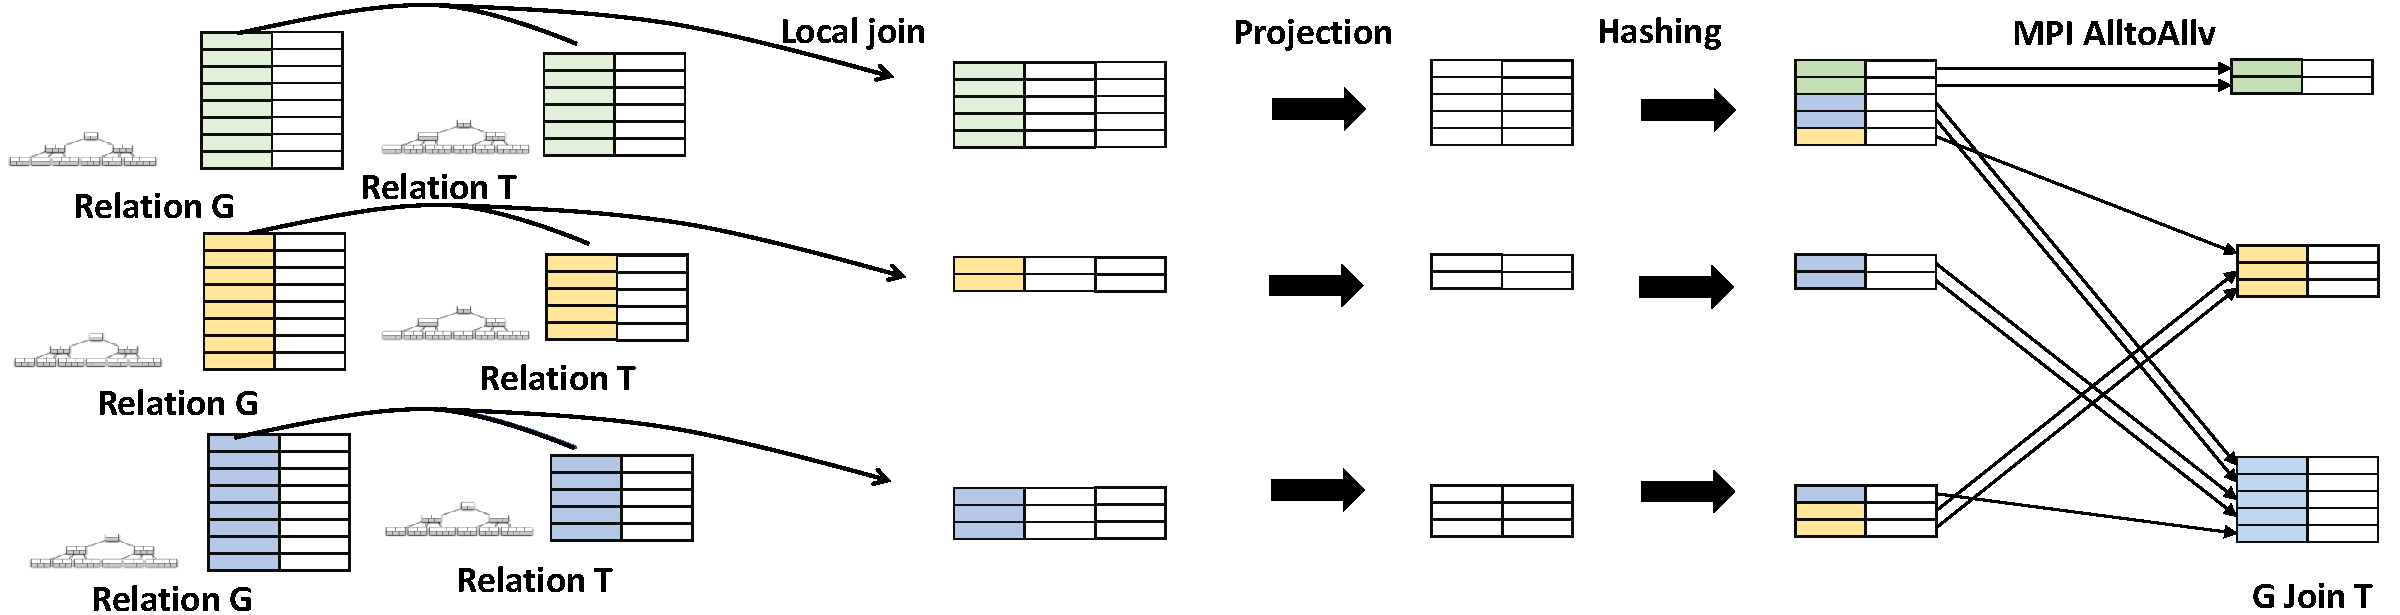
\includegraphics[width=\textwidth]{results/join_new.pdf}
	\caption{Schematic Diagram to show different phases of hash-tree join.}
	\label{fig:join}
\end{figure*}



\section{Hash-Tree Relational Algebra}
\label{sec:impl}
%
This section discusses our implementation of distributed relational algebra. We employ a hybrid approach we call \emph{hash-tree} relational algebra that consists of nesting B-tree key-value stores within a hash-table that can be partitioned across multiple cores or MPI nodes. As discussed in the previous section, the key-value store approach to encoding relations requires nested maps to support efficient join (and select) operations. In a typical join, it will be necessary to iterate over all tuples in a relation where particular columns match a value or values taken from the first operand of join---in which case the variable being matched should come first and be a key in the outermost B-tree. The relation is thus explicitly indexed on this column.

In our implementation, a relation $R(a,b)$ indexed on $a$ is encapsulated in a type \texttt{Relation<Relation<void>>} which provides an interface to a B-tree mapping \texttt{uint64\_t} keys, storing each $a$, to subrelations over just those values $b$ that are paired with a particular $a$. In our approach, this nesting of B-trees is extended at the top-level by a hash table so that each value $a$ is also hashed to one of $\mathit{nproc}$ (the number of MPI processes being used to host the relation) \textit{buckets}.

\paragraph{Hybrid join} The standard way to parallelize the key-value store approach to relational algebra on multi-core systems is to partition the iteration space of the outermost loop. For example, the Souffl\`e Datalog solver ~\cite{Scholz:2016:FLP:2892208.2892226} uses OpenMP to parallelize its join operations, first partitioning the outermost key-value store into multiple disjoint iterators---one for each available thread. Souffl\`e's join algorithm is nearly identical to our previous pseudocode for join, except that it adds an outer parallel for loop.   

\begin{verbatim}
      new_delta_path = {}
      pfor part_iter in delta_path.partition():
         for [x,y] in part_iter:
            for [y,z] in edge.select("y", y):
               if path.insert([x,z]) == true:
                  new_delta_path.insert([x,z])
      delta_path = new_delta_path   
\end{verbatim}


\subsection{Distributed hash-tree join}

Our hybrid hash-tree structure for relations makes this partitioning explicit as physically separate relations stored in distinct hash-table buckets---each owned by a dedicated MPI process. Join operations then decompose into a separate join for each bucket, followed by hashing of output tuples, and a communication phase to insert these tuples into the output relation. In experiments designing our join operation, we found that, as hashing distributes keys evenly across buckets, MPI's all-to-all communication paradigm was actually most efficient for inserting output tuples in their receiving buckets (i.e., on processes hosting the output relation).

In figure~\ref{fig:join} we show the process for computing a single iteration of a distributed transitive closure computation. $T$ (i.e., $T_\Delta$ as we implement an incrementalized TC algorithm) is joined with $G$ on a per-bucket basis (the diagram shows three color-coded buckets). Tuples in $T(x,y)$ are indexed on the second column ($y$) and tuples in $G(y,z)$ are indexed on the first column ($y$). This makes it possible to perform local (intra-bucket) joins as each tuple $(x,y) \in T$ is guaranteed to have all matching tuples $(y,z) \in G$ stored in the same bucket, managed by the same MPI process. Each resulting triple $(x,y,z)$ has its middle column projected out on-the-fly as it is produced, and, as the resulting tuple $(x,z)$ must be inserted into $T$, a relation indexed on its second column, each new edge is hashed and assigned to bucket $\mathit{hash}(z)\%\mathit{nprocs}$ in the output relation ($T$). As this bucket will likely not be managed by the local MPI process, a communication phase is required to actually perform insertion of each output tuple in its output relation. As each output tuple is produced it is staged in one of $\mathit{nprocs}$ packets, ready to be sent across the network to the MPI process managing its bucket. Finally, an all-to-all communication phase is used to reorganize the output of the join operation---preparing $T$ for subsequent fixed-point iterations. As tuples are received by their host process, they are inserted into the local B-tree structure, eliminating duplicates.  


\subsection{Distributed hash-tree union}

%\begin{figure*}[h]
%	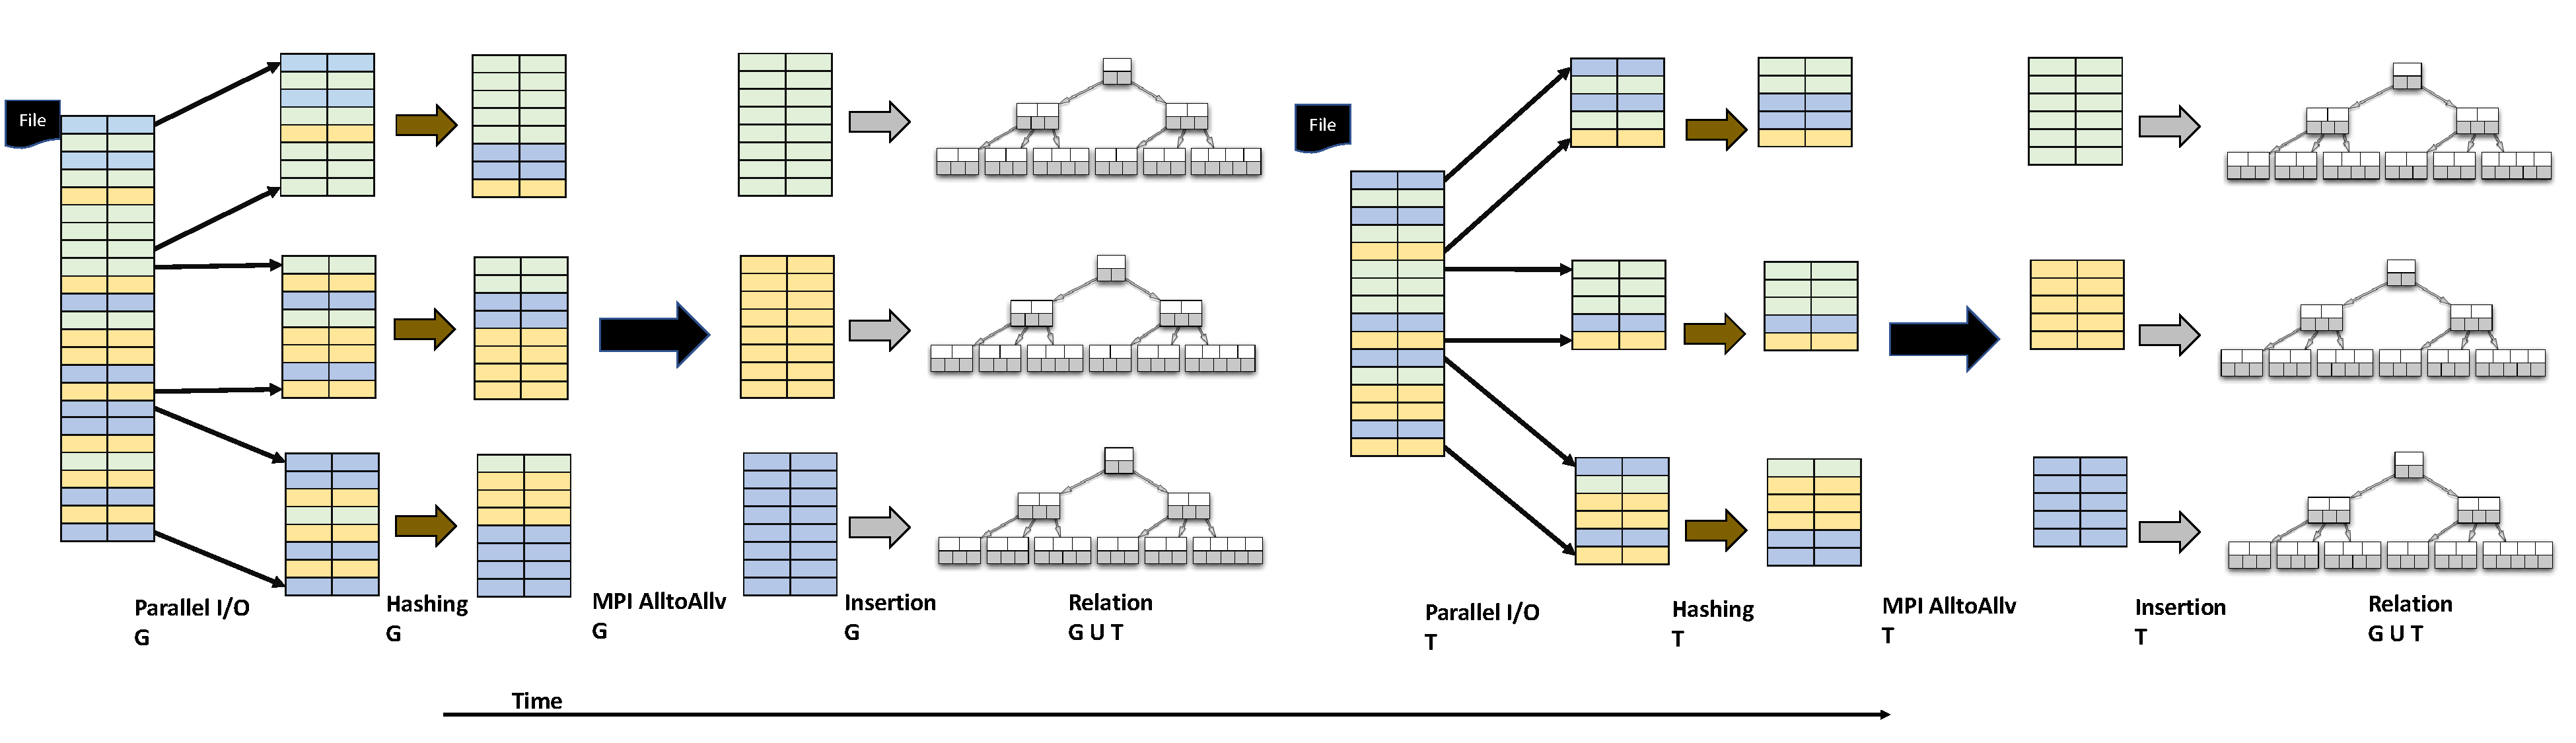
\includegraphics[width=\textwidth]{results/union_1.pdf}
%	\caption{Schematic Diagram to show different phases of naive hash-tree union.}
%	\label{fig:union_1}
%\end{figure*}

We present two algorithms for distributed unions, na\"ive hash-tree union and buffered hash-tree union. As the name suggests buffered hash-tree union buffers data across all relations that need to be unioned before performing any communication or insertions and performs the union concurrently in a single step. While performing a union of $n$ relations, na\"ive hash-tree union involves $n$ epochs of communication and computation---one for each relation---as opposed to buffered hash-tree union (see figure~\ref{fig:union_2}) that uses buffering to limit the number of communication and computation epochs to one.

Na\"ive hash-tree union is concurrent in processing each relation being unioned, but unions each relation in a separate step. Naturally, our buffered implementation has an extra memory overhead as opposed to the na\"ive implementation where all graphs that need to be unioned are processed one at a time, however it is more representative of real applications (such as Datalog, program analysis, etc) where each relation being unioned would have a set of nodes hosting it and tuples across multiple relations could all be transmitted and inserted into a new relation concurrently.

\begin{figure}[h]
	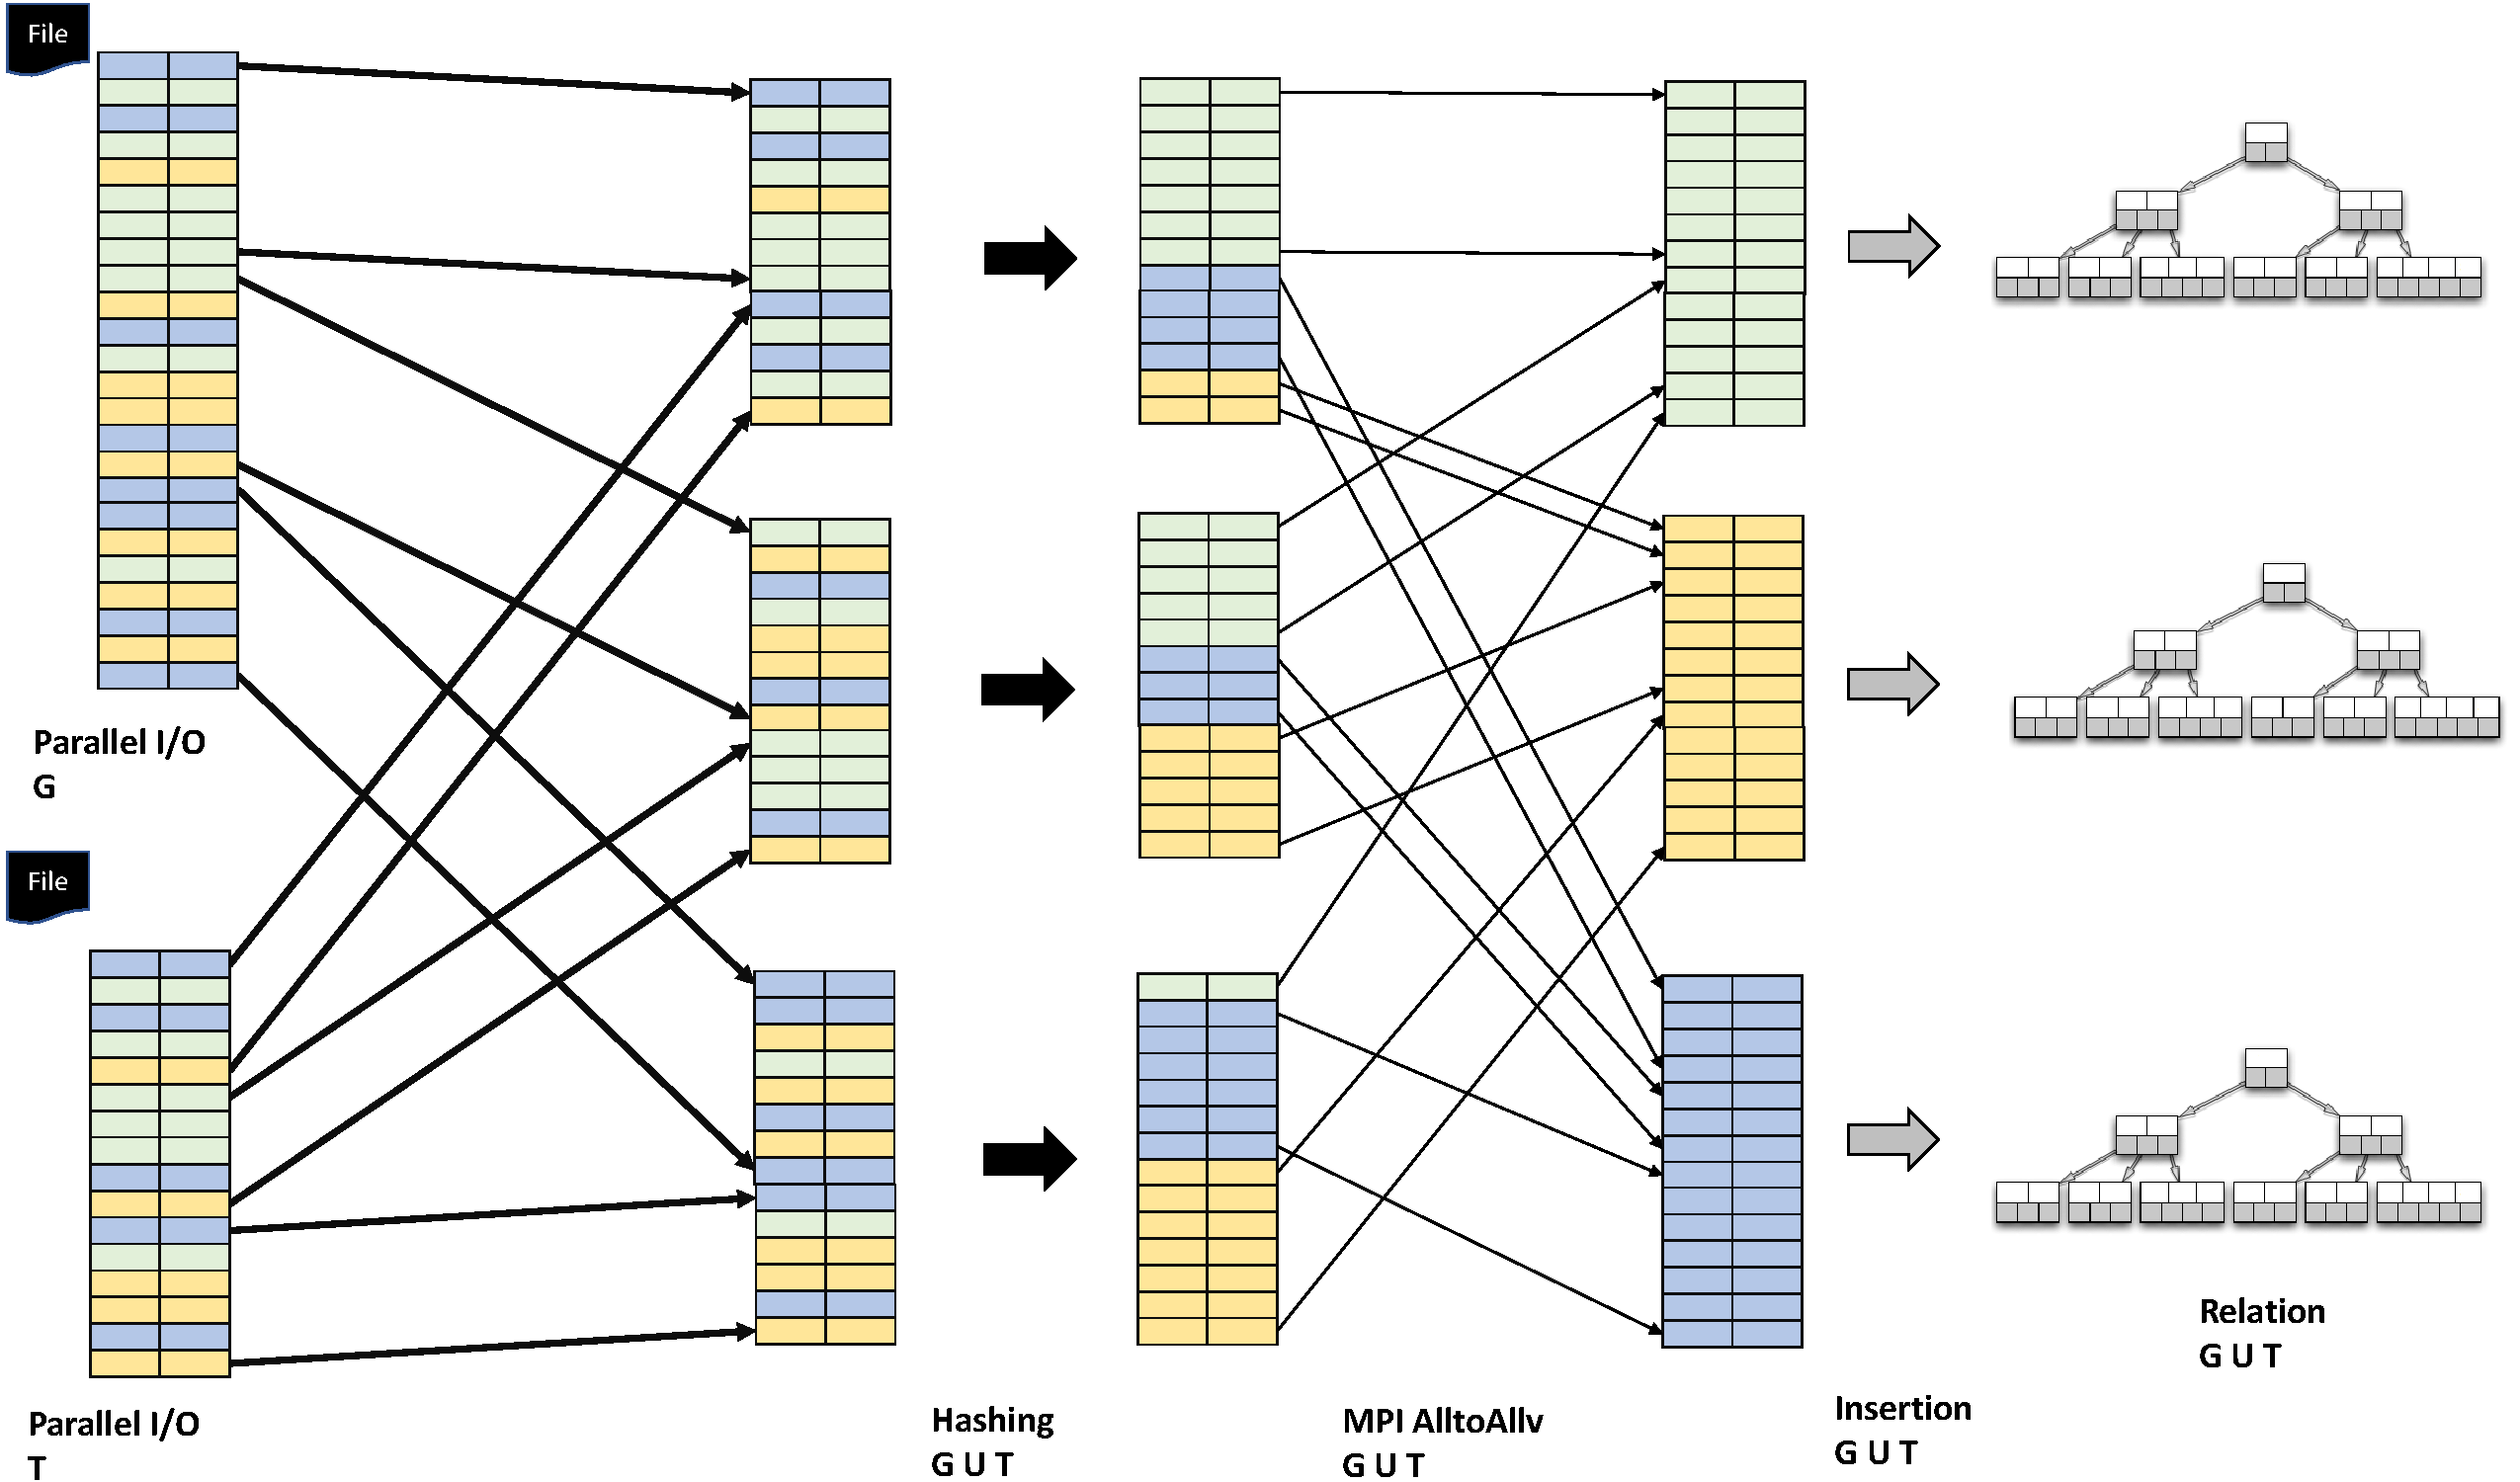
\includegraphics[width=\columnwidth]{results/union_2.pdf}
	\caption{Schematic Diagram to show different phases of buffered hash-tree union.}
	\label{fig:union_2}
\end{figure}

The input graphs can be read from files stored on the disk or can be read directly from memory. If the graphs are read from disk, the first phase is that of parallel I/O: processes access disjoint regions of the file to read an equal number of tuples in parallel. Once the tuples are read into memory, each process scans through its tuples and hashes them, grouping tuples into $\mathit{nprocs}$ packets, ready to be sent across the network. The target process (i.e., outer hash-bucket) of a tuple is computed based on the hash value of its key. For instance, the target rank of a two column tuple $(a, b)$, where $a$ is the outer key and $b$ the inner key, would be $\mathit{hash}(a)\%\mathit{nprocs}$. We also perform preliminary deduplication, as these tuples are staged, before transmitting these batches of tuples to minimize communication overhead. The grouping step is followed by an all-to-all communication phase where tuples are sent to the appropriate processes (outer hash buckets). Once tuples arrive at a process, they are inserted into the local relation container. This step performs the important task of deduplication of tuples across relations. 




\section{Evaluation}
\label{sec:eval}

%There are two goals of this sections 1) evaluate the performance of RA primitive operations Union and Join  2) evaluate the performance of transitive closure, which is a fixed point iteration algorithm.
The goal of this section is to evaluate the performance of our implementation of parallel join, parallel union and parallel transitive closure at scale.
We first individually study the computation and communication components of the RA operations.
Computation is dominated by insertion of tuples and the major challenge faced is that of deduplication.
We first study the efficacy of our btree-based relation container for inserts specifically in the context of deduplication.
All our RA operations involve an all to communication phase, hence, we perform a detailed benchmark of MPI's all to all communication capability.
Finally we benchmark the efficacy of parallel union, parallel join and parallel transitive closure over a wider range of graphs.
%We first study how our data structure performs, and how well are the all to all communication primitives are supported by super computers. More specifically, we study how fast can we insert into our btree based relation class, and how efficiently can it support the task of de-duplication. This is mostly studying the computation aspect of our algorithms. Next, with the all to all tests, we benchmark the communication aspect of our algorithms.


%Radix-hash join and merge-sort join are two of the most popularly used parallel implementations of the inner join operation. Both these algorithms involve partitioning the input data so that they can be efficiently distributed to the participating processes. For example, in the radix-hash approach a tuple is assigned to a process based on the hash output of the column-value on which the join operation is keyed. With this approach, tuples on both relations that share the same hash value are always assigned to the same process. For every tuple in the left-hand side of the join relation is matched against all the tuples of the right-hand side of the join relation. Fast lookup data-structures like hash tables, or radix-trees (TRIE) can be used to organize the tuples within every process. The initial distribution of data using hashing reduces the overall computation overhead by a factor of the number of processes (n).

%More recently (Barthels et al. 2015, 2017), there has been a concerted effort to implement JOIN operations on clusters using an MPI backend. The commonly used radix-hash join and merge-sort join have been re-designed for this purpose. Both these algorithms involve a hash-based partitioning of data so that they are be efficiently distributed to the participating processes and are designed such that inter-process communication is minimized. In both of these implementations one-sided communication is used for transferring data between process. With one-sided communication the initiator of a data transfer request can directly access parts of the remote memory and has full control where the data will be placed. Read and write operations are executed without any involvement of the target machine. This approach of data transfer involves minimal synchronization between particiapting processes and have been shown to scale better that traditional two-sided communication. The implementation of parallel join has shown promising performance numbers; for example, the parallel join algorithm of (Barthels et al. 2017) ran successfully at 4,096 processor cores with up to 4.8 terabytes of input data


\subsection{Dataset and HPC platforms}
\label{sec:datasets}
We have performed our experiments using SuiteSparse Matrix Collection available at ~\cite{}.
SuiteSparse Matrix Collection (formerly known as the University of Florida Sparse Matrix Collection), is a large and actively growing set of sparse matrices that arise in real applications. The Collection is widely used by the numerical linear algebra community for the development and performance evaluation of sparse matrix algorithms. 
For our experiments, we chose six graphs representing a wide range in terms of the number of edges. The last three graphs are the largest available graphs.
Transitive closure of a graph with $n$ edges can generate upto $n^2$ edges (a fully connected graph). More generally, the number of edges in the transitive closure of a graph depends on the connectivity of the input graph. We found our third graph with X edges to be the most connected; the transitive closure of the graph generated 260 billion edges, which is 3 terabytes in size.
%-- wide range in terms of number of edges
%-- The transitive closure of third graph generated 260 billion edges, which corresponds to 4 tera bytes of data.

\begin{table}[]
	\begin{tabular}{lllll}
		\begin{tabular}[c]{@{}l@{}}Input graph \\ edge count\end{tabular} & Union & Join & \begin{tabular}[c]{@{}l@{}}Transitive \\ Closure\end{tabular} & Graph name \\
		\hline
		412148                                                            & \checkmark      &      &                                                               &            \\
		2100225                                                           & \checkmark       &      &                                                               &            \\
		6291408                                                           & \checkmark       &      &                                                               &            \\
		59062957                                                          & \checkmark       &      &                                                               &            \\
		136024430                                                         & \checkmark       & \checkmark     &                                                               &            \\
		180292586                                                         & \checkmark       & \checkmark      &                                                               &            \\
		240023949                                                         & \checkmark       &      &                                                               &           
	\end{tabular}
\end{table}


The experiments presented in this work were performed on
Theta at the Argonne Leadership Computing Facility
(ALCF). Theta is a Cray XC30 with a peak
performance of X petaflops, 124, 608 compute cores, 332
TiB of RAM, and 7.5 PiB of online disk storage. We used
Edison Lustre file system (168 GiB/s, 24 I/O servers and 4
Object Storage Targets). 

%Default striping was used with the Lustre file system. Mira system contains 48 racks and 768K cores, and has a theoretical peak performance of 10 petaflops. Each node has 16 cores, with 16 GB of RAM per node. I/O and interprocessor communication travels on a 5D torus network. Every 128 compute nodes has two 2 GB/s bandwidth links to two different I/O nodes, making 4 GB/s bandwidth for I/O at most. I/O nodes are connected to file servers through QDR IB. Mira uses a GPFS file system with 24 PB of capacity and 240 GB/s bandwidth.


\begin{figure*}[t]
	{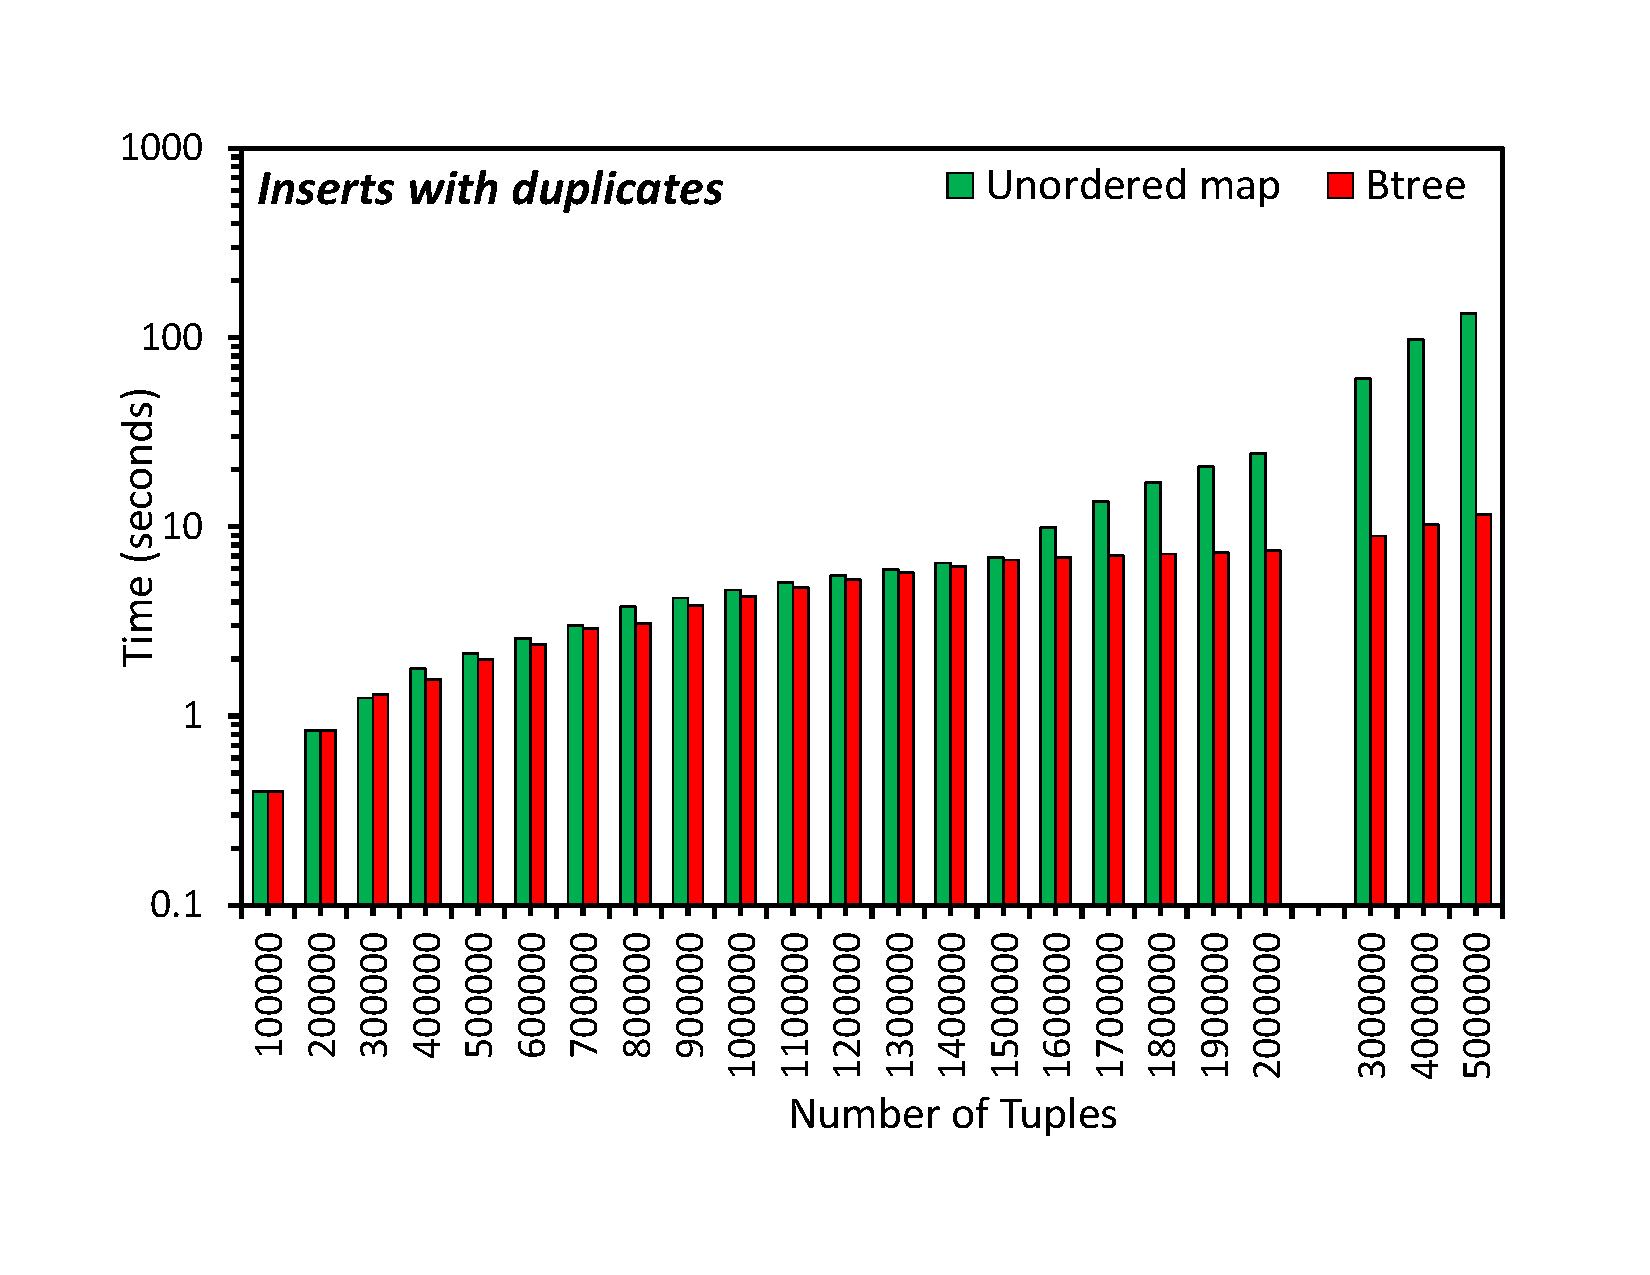
\includegraphics[width=.50\textwidth,  trim={0cm 0cm 0cm 0cm, 
			clip}]{results/inserts_with_duplicates.pdf}}\hfill%
	{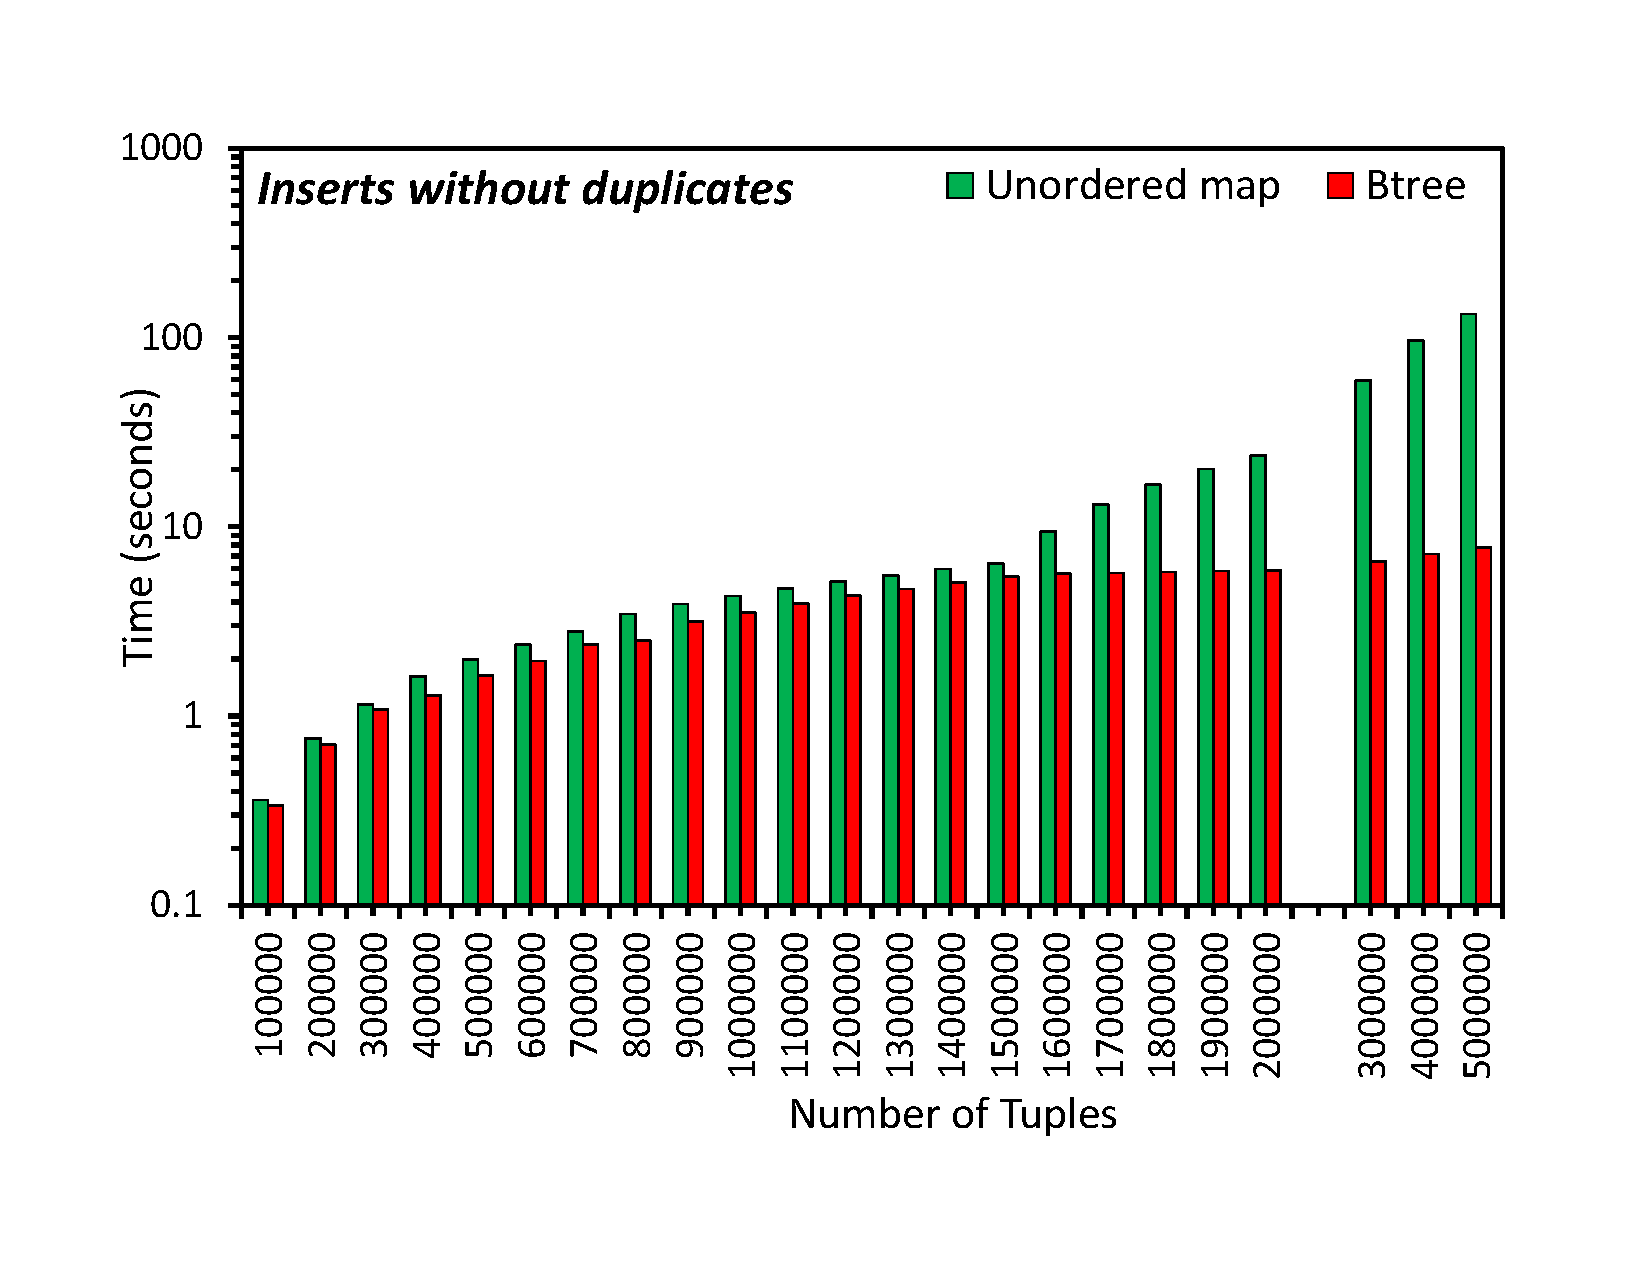
\includegraphics[width=.50\textwidth,  trim={0cm 0cm 0cm 0cm,
			clip}]{results/inserts_with_no_duplicates.pdf}}\hfill%
	\centering
	\caption{Performance evaluation of relation class implemented with btree and unordered map. (left) All tuples are distinct, (right) There are four copies of every tuple being inserted. Relation implemented with btree out-performs the unordered-map implementation.}
	\label{fig:tuple_inserts}
\end{figure*}


\subsection{Btree-Relation container}
\label{sec:relation}

In this section we evaluate the efficacy of our relation container.
We measure performance for two cases: insertions of unique tuples and insertions of tuples with duplicates. With the later set of experiments, every tuple had four duplicates. For both set of experiments, we compare two implementations of the relation class, one with a Btree back-end and the other with an hash map back-end. For the hash map, we used unordered\_map from C++'s standard template library. The results can be seen in Figure~\ref{fig:tuple_inserts}. The X-axis corresponds to the total number of tuples being inserted and the Y-axis is the time taken for the task to finish. We observe that btree-based relation container outperforms the hash map based implementation for insertion of all tuple counts. Furthermore hash map based relation container fails to scale with insertion of very large number of tuples. For example hash based relation takes X seconds to insert Y tuples as opposed to only Z seconds taken by btree based relation. Similar results can be observed for insertion of tuples with duplicates. The btree based relation container successfully dedeuplicate tuples while maintaining high performance.
%To facilitate fast inserts and lookups of tuples, we implemented a relation container.
%We made two implementations of the container one using btrees and other using unordered\_map from the standard template library.
%The relation container is a recursive, nested data-structure. \textbf{More stuff.}
%, for example, for two-tuple we have a btree with keys as the first column-entries, and the value is a new btree which is again
%Deduplication is a major challenge while inserting tuples, for example, join between two relation followed by projection of the common column often yields a lot of duplicate tuples. 


%-- Perform two benchmarks: insertion of tuples without any duplicate and insertion of tupes each with four duplicates.
%-- Relation class implemented with btrees outperforms relation with hashes.
%-- 



\begin{figure*}[t]
	{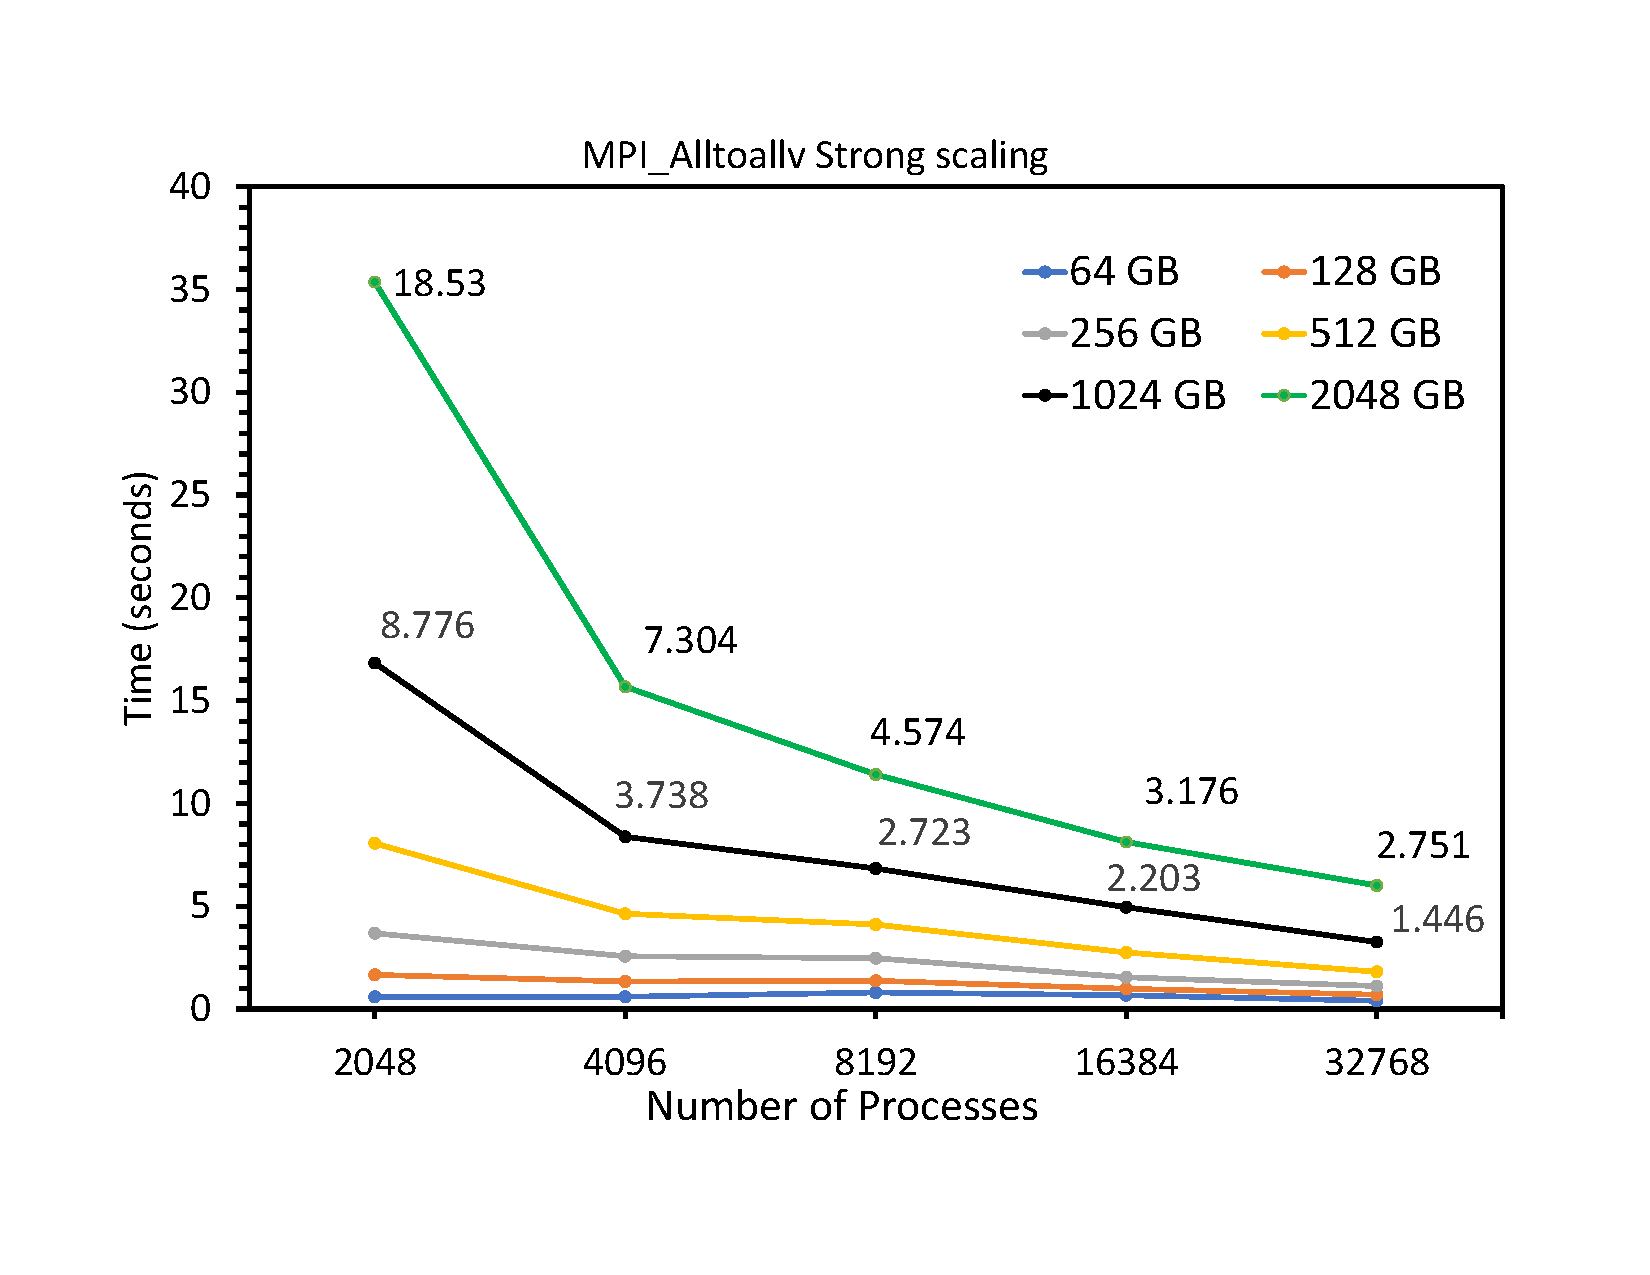
\includegraphics[width=.50\textwidth,  trim={0cm 0cm 0cm 0cm, 
			clip}]{results/all_to_all_strong.pdf}}\hfill%
	{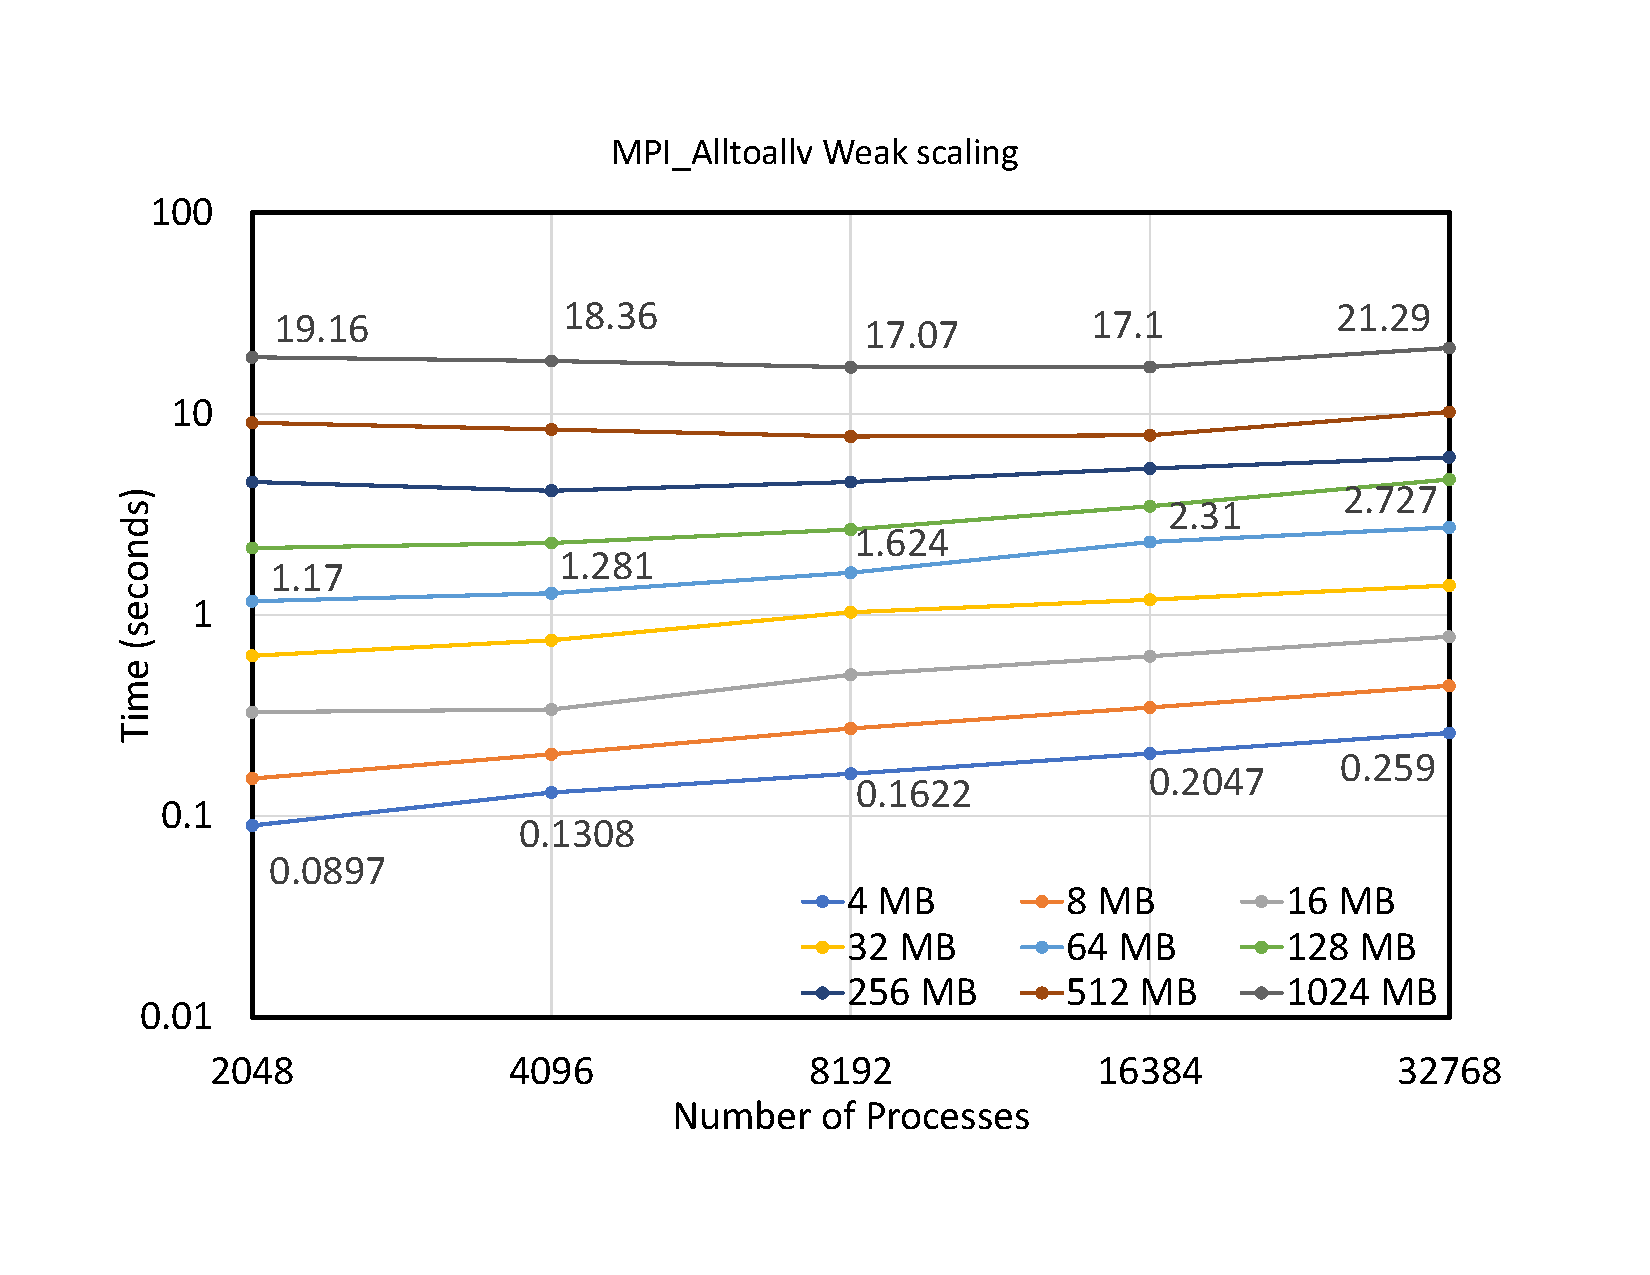
\includegraphics[width=.50\textwidth,  trim={0cm 0cm 0cm 0cm,
			clip}]{results/all_to_all_weak.pdf}}\hfill%
	\centering
	\caption{Strong (left) and Weak (right) scaling evaluation of MPI\_alltoallv function of MPI.}
	\label{fig:all_to_all}
\end{figure*}


\subsection{MPI\_All\_to\_Allv}
\label{sec:all_to_all}


%All our RA operations require all to all communication.
All to all communication forms the core of all our RA algorithms (\textbf{refer to the algorithms}).
We use MPI's MPI\_Alltoallv function to facilitate all to all data communication.
MPI\_Alltoallv sends data from all to all processes where each process can send a different amount of data by providing displacements for the input and output data. In this section we study both weak and strong scaling characteristics of MPI\_Alltoallv.
For both set of experiments, we varied the number of processes from $2048$ to $32768$. We performed 9 set of weak scaling experiments. For these 9 set of experiments, the amount of data transmitted by each process ($data_{process}$) was varied from 4 megabytes (1st set) to 1024 megabytes (9th set). For a $n$ process run, every process transmits $data_{process}/n$ units of data to every other process. With strong scaling experiments, we performed 6 set of experiments, varying the total amount of data generated across processes ($data_{total}$) from 64 gigabytes (1st set) to 2048 gigabytes (6th set). The amount of data generated by every process is the same, for example for a $n$ process run, and $data_{total}$ total amount of data, every process produces $data_{total}/n$ units of data. A process then transmits $data_{total}/n^2$ units of data to every other process.  The results of both weak and strong scaling experiments can be seen in Figure~\ref{fig:all_to_all}.

For both strong and weak scaling runs, we observe a decline in performance with decreasing workload. For instance, with strong scaling, the 6th set of experiments where total workload is 2048 gigabytes, we observe near perfect scaling when the number of processes is doubled from 2048 (18.5 seconds) to 4096 (7.3 seconds) to 8192 (4.5 seconds). After 8192 processes, although total time continues to come down with increasing process count, we observe that the rate becomes much slower. Furthermore, looking at the 6th set of experiments where total workload is 64 gigabytes we observe relatively poor scaling characteristics across the entire process range. Both the observations can be attributed to reduced per-process workload. With less amount of data to transmit, total time is dominated by initialization costs as opposed to data transmission costs. Similarly for weak scaling experiments as well, when the amount of data exchanged is substantial, we see almost perfect scaling. For example, when the amount of data transmitted by every process is 1024 megabytes, we observe almost perfect scaling, whereas when the amount of data sent by every process is small (4MB) we observe poor scaling.


With the context of communication requirements of RA operations, we find the scaling trends of MPI\_alltoallv to be encouraging. In general for a given workload (graph size for RA operations), there will always be a range of processes that exhibits good all to all scaling characteristics. We will have the challenging task to identify the right process count that balances the tradeoff between computation and communication. As we will see later in section~\ref{sec:tc} with larger per-process load computation cost dominates as opposed to smaller per-process workload where total cost is dominated by communication. 
%As we will ee later the crucial part will be to identify the process count that balances computation and communication in the monst efficient way.

%For every input graph, we need to find the range of process count that exhibits 
%The trends suggests that there is a range of process count suitable for different graphs. There is a window of process count suitable for graphs of differeing sizes. As the number of processes increases the amount of data (tuples) held by every process starts t

%-- perform both weak and strong scaling
%-- configuration
%-- weak scaling with accuracy X percent accuracy for per process load of Y versus Z percent accuracy for per process load of M.
%-- Exhibit poor weak scaling for small load, as opposed to good weak scaling with larger volume of data.
%-- X percent accuracy with strong scaling of X load. This corresponds to Y number of tuples.
%-- Overall very good indication as all to all scales well, aggregate accuracy
%-- different graphs would work better at different scales.

\subsection{Distributed Union}
\label{sec:union}

\begin{figure*}[t]
	{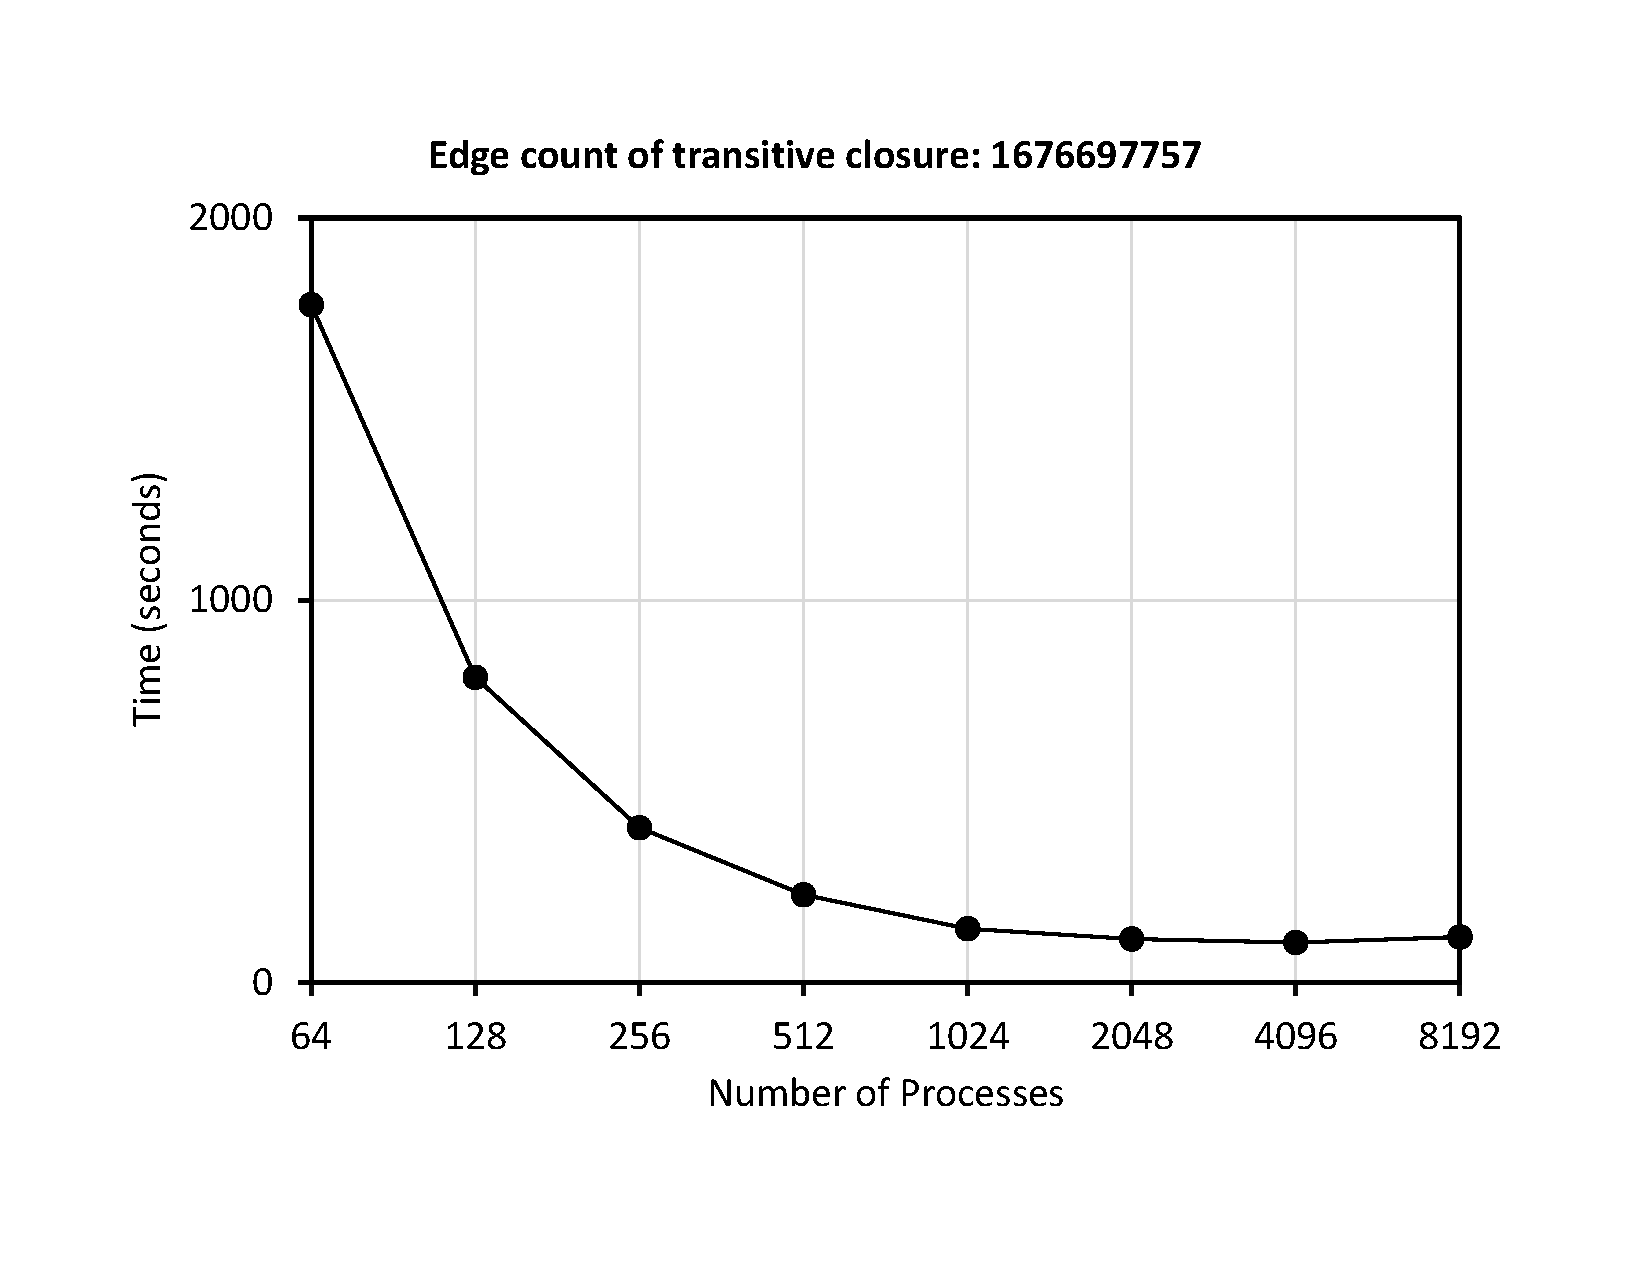
\includegraphics[width=.50\textwidth,  trim={0cm 0cm 0cm 0cm, 
			clip}]{results/TC_1_6Billion.pdf}}\hfill%
	{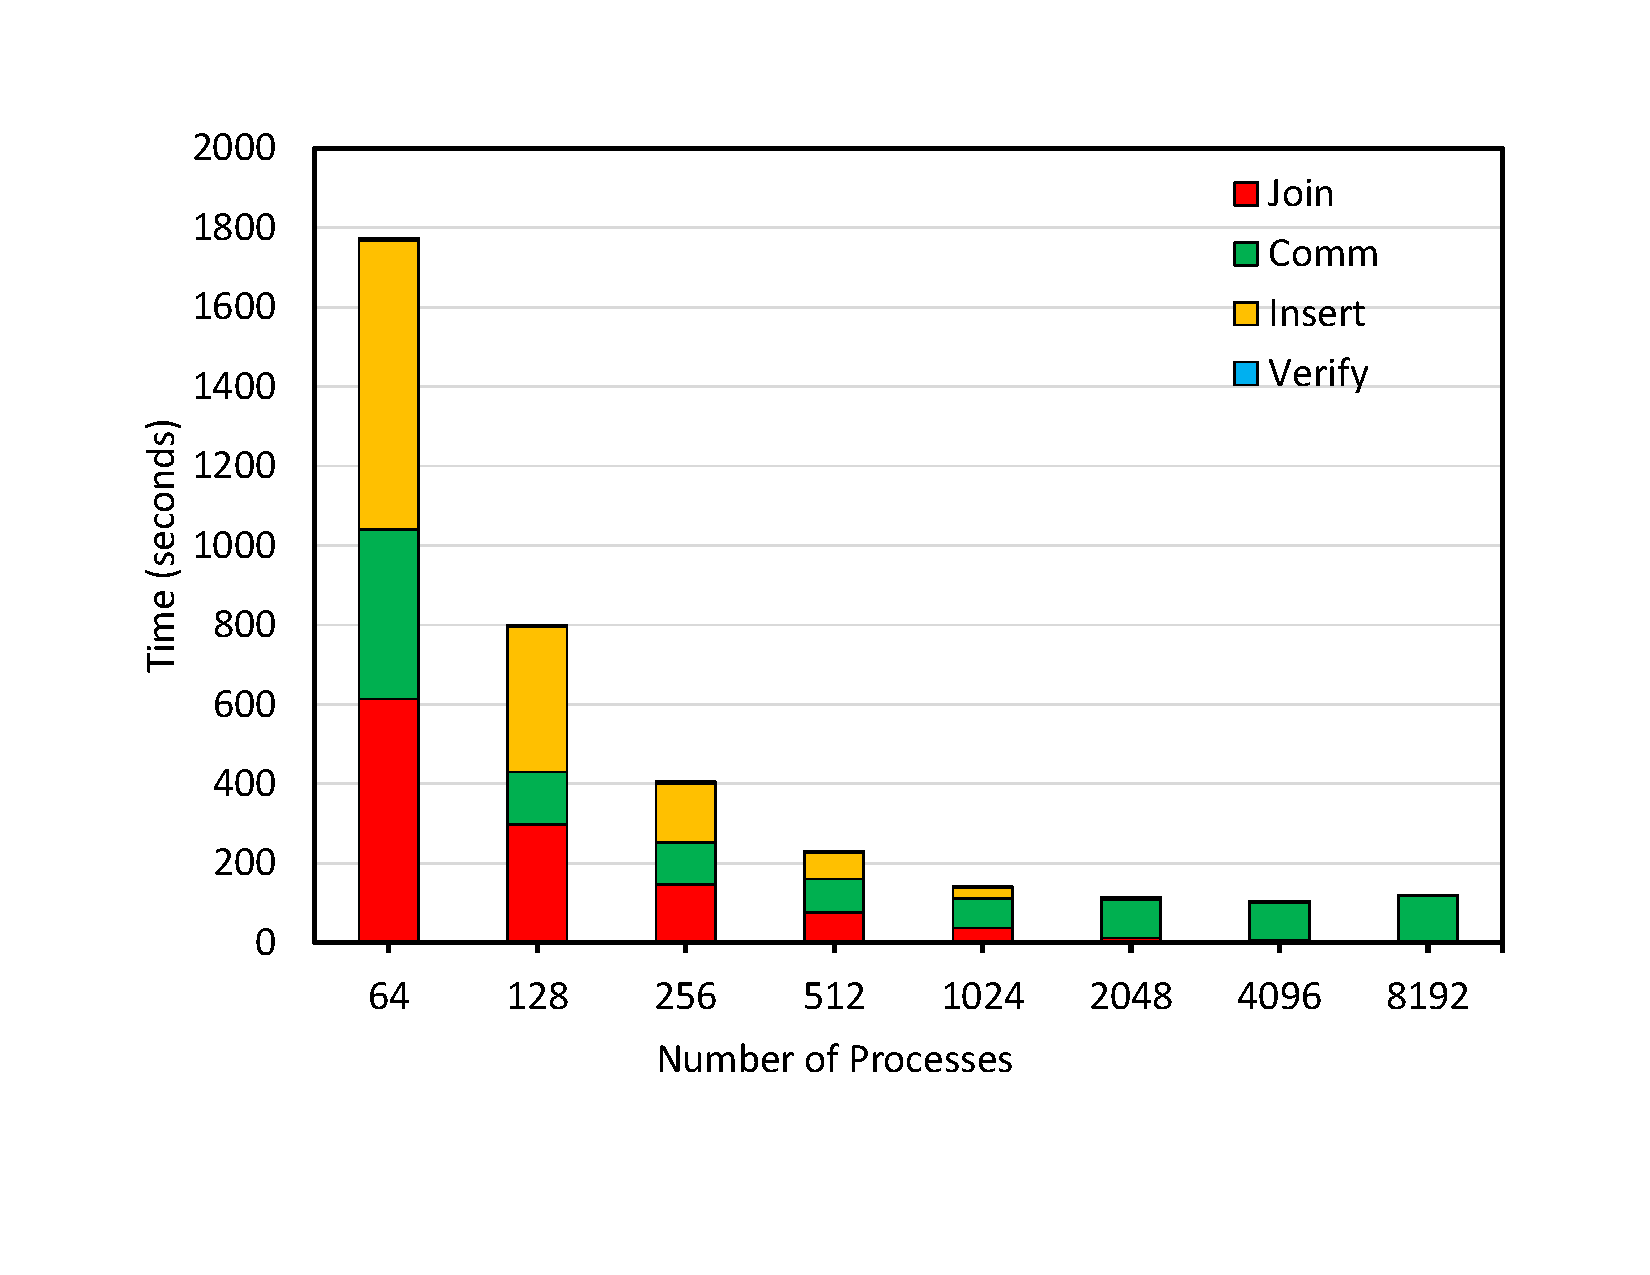
\includegraphics[width=.50\textwidth,  trim={0cm 0cm 0cm 0cm,
			clip}]{results/TC_1_6Billion_breakdown.pdf}}\hfill%
	\centering
	\caption{Transitive closure of a graph with X edges.}
	\label{fig:tc_small}
\end{figure*}

We use strong scaling to benchmark the performance of distributed union operation. We measure the timing to perform union of all 7 graphs listed in table~\ref{table:graphs}. The number of processes are varied from $64$ to $4,096$. The total number of edges across all $7$ graphs is $664,659,334$ ($~9.9$ gigabytes of data). Union of the seven graphs result in a graph with $424,592,810$ edges, indicating significant overlap between the graphs.

We benchmark the performance of both union\_x and union\_y. Union\_x involves seven epochs of communication and computation (one for every graph) as opposed to union\_y that uses buffering to limit the number of communication and computation epochs to one. With union\_x, all processes iterate through all seven graphs. The first phase is that of parallel I/O, where processes access disjoint regions of the file to read equal number of tuples in parallel. Once the tuples are read, every process scans through the tuples and groups them into $nprocs$ (=$hashbuckets$) packets, ready to be sent across the network.
Target process (hash-bucket) of a tuple is computed based on the hash outcome of its key. For instance, target rank of a two column tuple $(a, b)$ would be $hash(a)\%nprocs$. We also perform preliminary deduplication to eliminate duplicate tuples in the input graph. The scan step is followed actual by all to all communication phase where tuples are sent to the appropriate processes (hash buckets). Once tuples arrive at a process, they are inserted into the relation container. This step performs the important task of deduplication of tuples across the graphs. 

With union\_y instead of processing the graphs one after the other, we read all the graphs at once, buffer the tuples and follow it with one cumulative step of hashing, communication and insertion. This implementation deploying buffering restricts the number of communication epochs. Performance of both implementation can be seen in Figure~\ref{fig:parallel_union}. For both implementations, we present breakdown of time spent in each of the three phases: parallel I/O, all-to-all communication and insertions. We observe two trends: at all core counts, union\_y outperforms union\_x, this trend can be attributed to an optimized data communication phase. Union\_y leads to communication involving small number of large sized data packets as opposed to union\_x that involves communication with large number of small sized data packets. The other crucial trend is that the union phase scales only till 1024 cores, this can be attributes to increase in communication time at higher core counts. This result is in corroboration with the trend seen in Section~\ref{sec:datasets}. At 2048 and 4096 processes, even though the insertion time gets reduced, the per-process workload becomes very small impeding scalability of the communication phase. It can be concluded that for this particular union task ($7$ graphs) $1024$ is the ideal degree of parallelism, as that balances the communication and computation task best.

%This step is followed by 

%-- union of 7 graphs from table
%-- union comprises of an io phase followed by communication and then followed by inserts
%-- We compare two union types, one is where we perform io, comm and compute separates, the other is where we first perform io for all and then we bundle all our comm and then we have one phase of compute
%-- scales well upto X cores., this is strong scaling.
%-- faces work load deprecation at low core counts, needs more tuples for union to scale at high core counts
%-- overall a good sign


\subsection{Distributed Join}
\label{sec:join}
Similar to distributed union, we use strong scaling to benchmark the performance of distributed join as well.
We perform join of two graphs with edges $136,024,430$ and $180,292,586$. The join operation yields a graph with X number of edges.
The number of processes are varied from $64$ to $4,096$. 
%Unlike union, where we maintained only one relation container for all input graphs, here we have separate relation containers for the two input graphs. 
Once the two relations are initialized across all processes (after parallel I/O, hashing, communication and insertions), we initiate the join operation. 
We plot the result of join operation in Figure~\ref{fig:join}. We observe trends similar to distributed union.
Join only scales upto X cores, after which communication cost starts to dominate and we observe overall decline in performance.


\subsection{Transitive closure}
\label{sec:tc}

Computing the transitive closure of a graph involves repeated join operations until a fixed point is reached. 
Iteration ($i$) adds new paths of length $i$, until a fixed point is reached and no new edges are added.
We use the hash-join (\textbf{TODO: refer} to distribute the tuples across all processes.
Every iteration comprises of four phases: 1) Join 2) network communication 3) insertion 4) checking for a
fixed point. In the join phase every process concurrently computes the join of relations $G$ and $T = \rho_{0 / 1}(G)$ which creates new edges. Following the semi-naive evaluation (discussed in Section~\ref{}), the new edges are then added back to relation $T$. This step of adding newly created edges entail all to all communication. The new edges need to be rehashed and sent to appropriate hash-buckets (processes). 
We accomplish this all-to-all communication using MPI’s MPI\_alltoallv routine where newly created edges are transmitted to all the processes.
Following the insertion phase, the newly created edges are inserted to the relation T.
In the final step we check if the size of the relation $T$ changed on any process, if it does then we have not yet reached a fixed point and we continue to
another iteration of these 4 steps.


We performed a set of strong-scaling experiments to compute the transitive closure of graph with 412148
edges—the largest graph in the U. Florida Sparse Matrix set (Davis and Hu 2011). We used the Quartz supercomputer
at the Lawrence Livermore National Laboratory (LLNL). For our runs, we varied the number of processes
from 64 to 2048. A fixed point was attained after 2933 iterations, with the resulting graph containing 1676697415
edges. As can be seen in Figure 1, our approach takes 462 seconds at 64 cores and 235 seconds at 2048 cores, corresponds
to an overall efficiency of 6.25%. We investigated these timings further by plotting the timing breakdown
of by the four major components (join, network communication, join, fixed-point check) of the algorithm. We
observe (see Figure 2) that for all our runs the total time is dominated by computation rather than communication;
insert and join together tended to take up close to 90% of the total time. This is quite an encouraging result
as it shows that we are not bound primarily by the network bandwidth (at these scales and likely moderately
higher ones) and it gives us the opportunity to optimize the computation phase

\begin{figure*}[t]
	{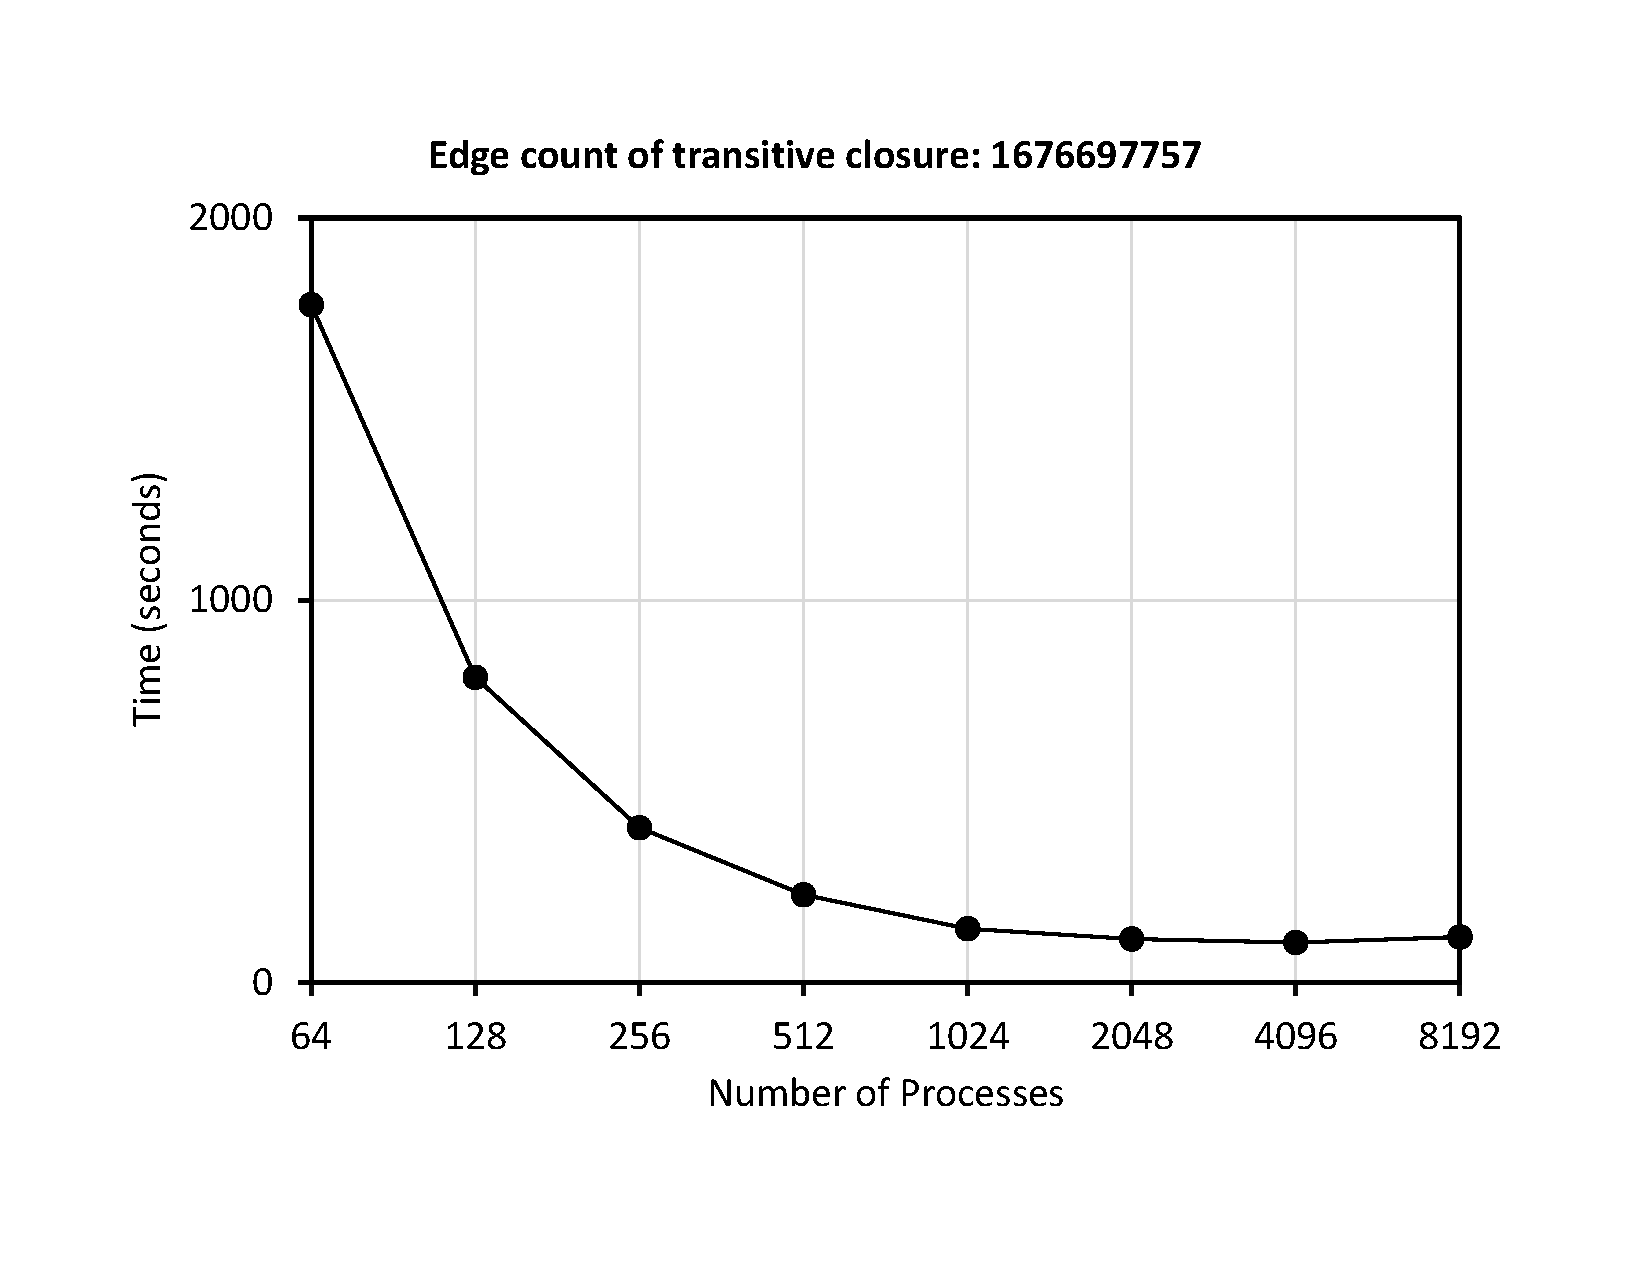
\includegraphics[width=.50\textwidth,  trim={0cm 0cm 0cm 0cm, 
			clip}]{results/TC_1_6Billion.pdf}}\hfill%
	{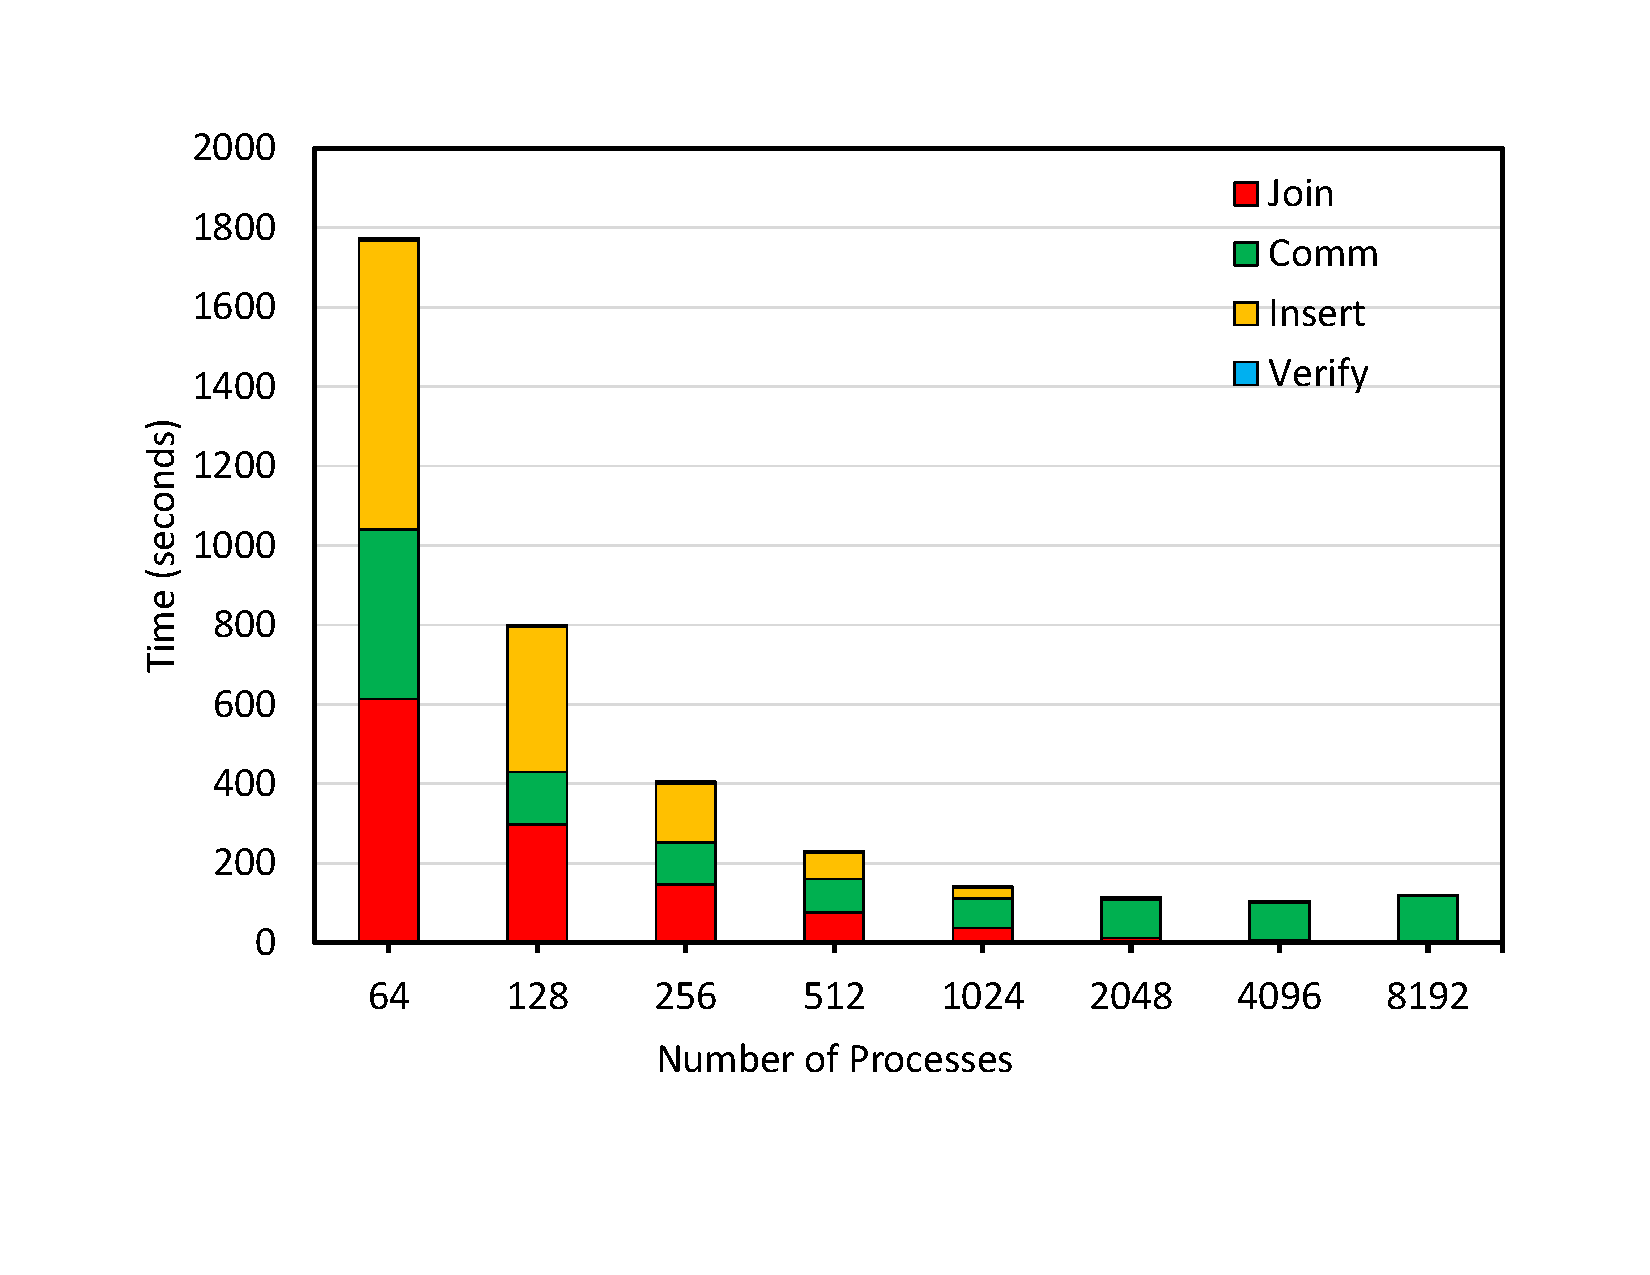
\includegraphics[width=.50\textwidth,  trim={0cm 0cm 0cm 0cm,
			clip}]{results/TC_1_6Billion_breakdown.pdf}}\hfill%
	\centering
	\caption{Transitive closure of a graph with X edges.}
	\label{fig:tc_small}
\end{figure*}


\begin{figure*}[t]
	{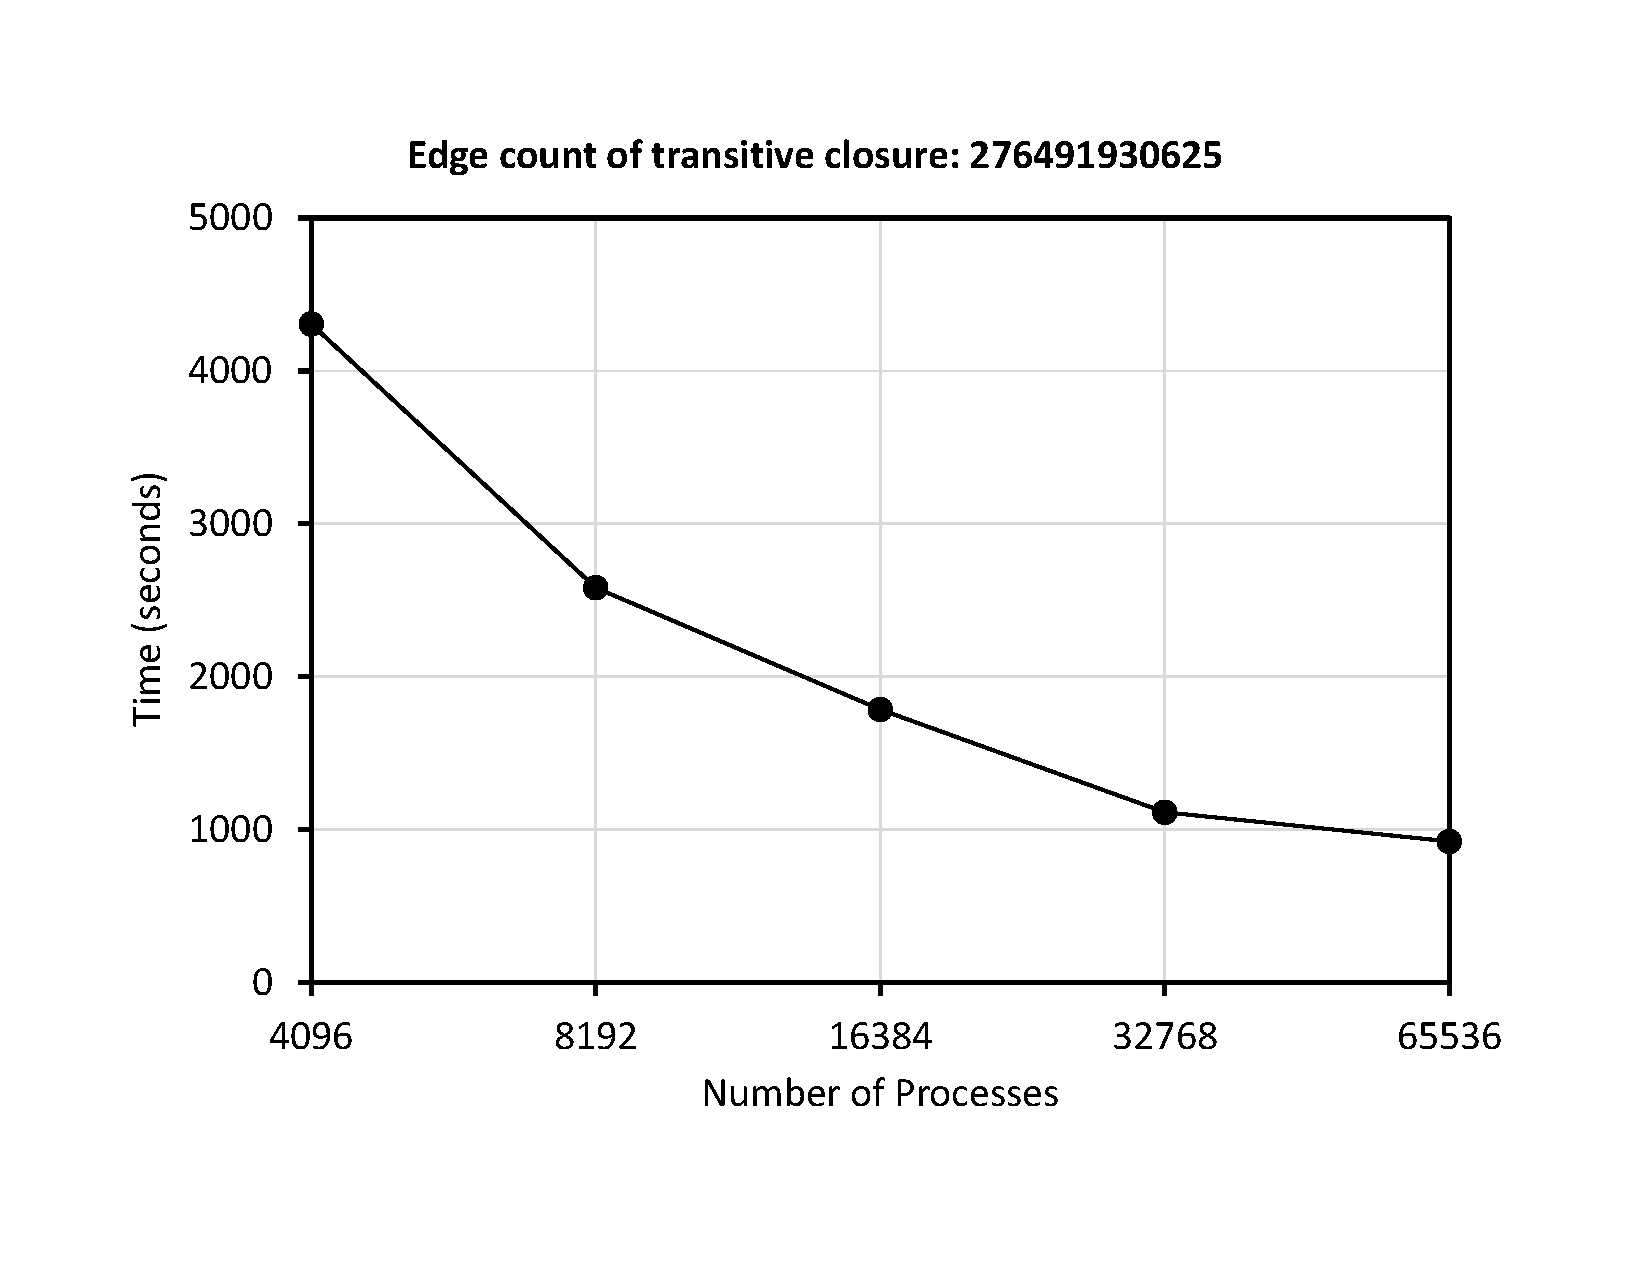
\includegraphics[width=.50\textwidth,  trim={0cm 0cm 0cm 0cm, 
			clip}]{results/TC_260Billion.pdf}}\hfill%
	{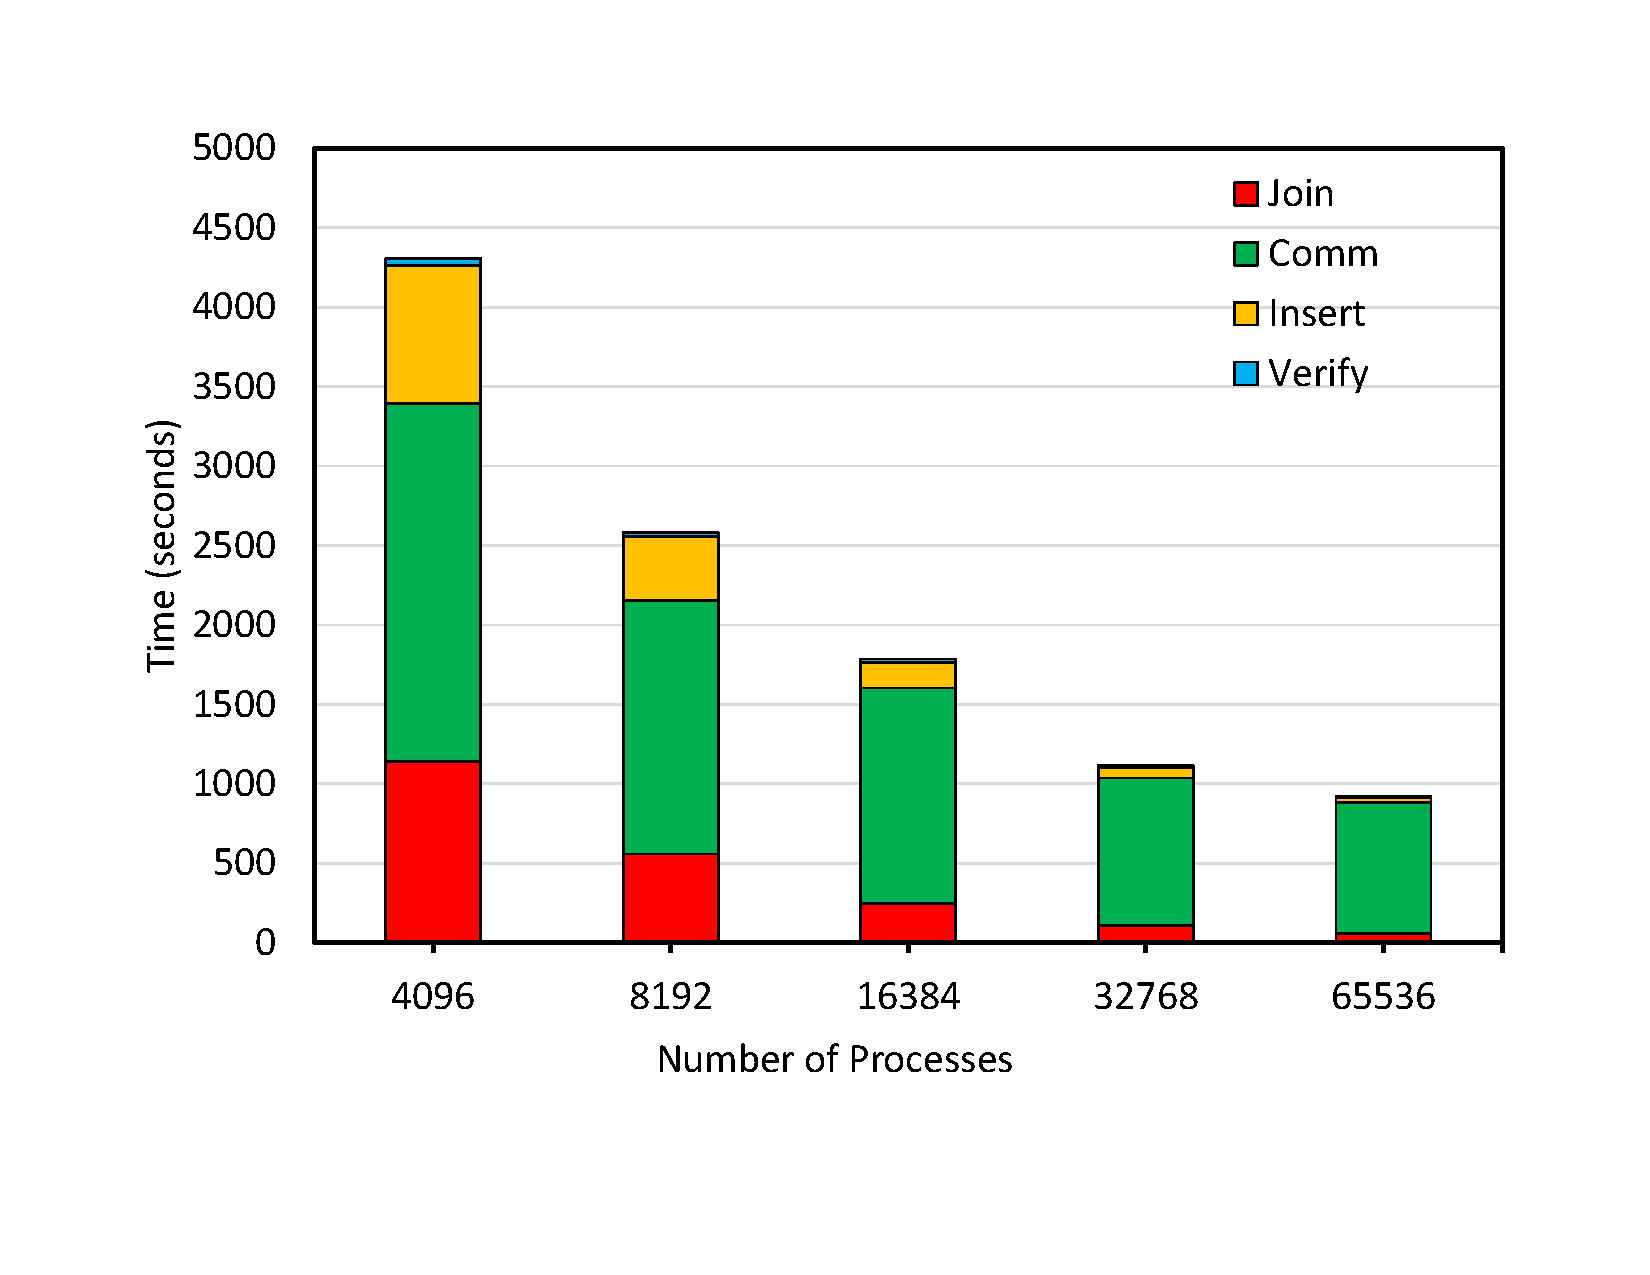
\includegraphics[width=.50\textwidth,  trim={0cm 0cm 0cm 0cm,
			clip}]{results/TC_260Billion_breakdown.pdf}}\hfill%
	\centering
	\caption{Transitive closure of a graph with X edges.}
	\label{fig:tc_large}
\end{figure*}


\section{Related Work}
\label{sec:related}
%
Lorem ipsum dolar sit amat 





\section{Conclusion}

We have presented the first general algorithms for scalable relational algebra on supercomputers. Our approach addresses both representation and communication among portions of a distributed relation, laying the groundwork for scaling algorithms that require a pipeline of repeated operations on relations, or fixed-point iteration, such as logical and constraint problems, deductive databases, and static program analyses. We discovered that MPI's all-to-all communication paradigm is scalable, and suitable for relational algebra. Finally, we demonstrated the scalability of our operations, up to $65,\!536$ nodes, in the context of a fixed-point algorithm for computing transitive closure.

In future work, we plan to address distributing relations via hashing on multiple variables to improve performance for highly non-uniform relations. We also have plans to address combining task-level and data-level parallelism in the context of Datalog solvers---a problem that must naturally extend to large numbers of relations and fixed-point interation over equally large numbers of constraints.




%\begin{acks}
%To Robert, for the bagels and explaining CMYK and color spaces.
%\end{acks}

%

% The next two lines define the bibliography style to be used, and the bibliography file.
%\bibliographystyle{ACM-Reference-Format}
\bibliographystyle{abbrv}
\bibliography{sample-base}

% 
% If your work has an appendix, this is the place to put it.
%\appendix


\end{document}
